\documentclass[a4paper,10pt]{article}
\usepackage[polish]{babel}
\usepackage[utf8]{inputenc}
\usepackage{polski}
\usepackage[T1]{fontenc}
\usepackage{enumerate}
\usepackage{indentfirst}
\usepackage{graphicx}
\usepackage{fancyhdr}
\usepackage{minted}
\usepackage[pdftex,pagebackref=false,draft=false,pdfpagelabels=false,
colorlinks=true,urlcolor=blue,linkcolor=red,citecolor=green,pdfstartview=FitH,
pdfstartpage=1,pdfpagemode=UseOutlines,bookmarks=true,bookmarksopen=true]{hyperref}


\setlength{\textheight}{24cm}
\setlength{\textwidth}{15.92cm}
\setlength{\footskip}{10mm}
\setlength{\oddsidemargin}{0mm}
\setlength{\evensidemargin}{0mm}
\setlength{\topmargin}{0mm}
\setlength{\headsep}{5mm}

\definecolor{code}{rgb}{0.95,0.95,1}

\renewenvironment{description}[1][0pt]
	{\list{}{\labelwidth=0pt \leftmargin=#1
	\let\makelabel\descriptionlabel}}
	{\endlist}

\author{Mateusz Gałażyn, Jeremi Niedziela}
\title{Krótki kurs tworzenia stron w technologii PHP}


\frenchspacing
\begin{document}

\pagestyle{fancy}
\lhead{Krótki kurs tworzenia stron w technologii PHP}


\maketitle
\section{Wstęp}
Ten krótki kurs ma na celu przedstawienie sposobu pisania stron przy użyciu technologii Apache + MySQL + PHP (w skrócie AMP) - jednego z najpopularniejszych zestawów oprogramowania służącego do uruchamiania serwisów WWW. Ten kurs jest bardzo okrojony i zawiera tylko wybrane elementy języka PHP oraz MySQL dlatego aby w pełni zrozumieć metodykę tworzenia aplikacji w oparciu o te  języki dobrze jest się wspierać dokumentacjami technicznymi, innymi kursami dostępnymi w internecie, a także specjalistycznymi forami dyskusyjnymi. \\
Dokumentacja PHP: \href{http://www.php.net/manual/pl/}{http://www.php.net/manual/pl/} \\
Dokumentacja MySQL: \href{http://dev.mysql.com/doc/refman/5.5/en/index.html}{http://dev.mysql.com/doc/refman/5.5/en/index.html} \\
Dokumentacja Apache: \href{http://httpd.apache.org/docs/2.4/}{http://httpd.apache.org/docs/2.4/} \\
Kurs PHP @ Wikibooks: \href{http://pl.wikibooks.org/wiki/PHP}{http://pl.wikibooks.org/wiki/PHP}

\subsection{Mechanizm działania systemu AMP} 
Gdy użytkownik strony uruchamia przeglądarkę i wpisuje w pasek adresu, adres szukanego serwisu WWW, przeglądarka nawiązuje połączenie z serwerem na którym są uruchomione usługi umożliwiające dostęp do strony. \\
\textbf{Apache} - jest to najszerzej stosowany w internecie serwer HTTP \\
\textbf{PHP} - jeden z najpopularniejszych języków programowania używany do tworzenia stron WWW. \\
\textbf{MySQL} - system zarządzania bazami danych za pomocą języka SQL \\


\begin{figure}[htbp]
\centering
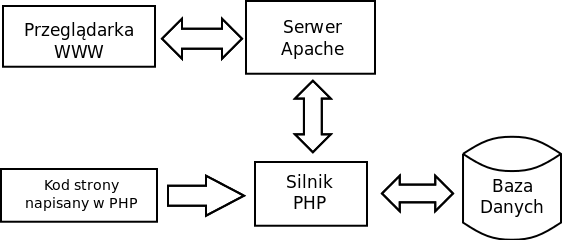
\includegraphics[width=0.7\textwidth]{LAMP.png}
\caption{Schemat komunikacji zestawu AMP}
\end{figure}

Żądanie otrzymane od przeglądarki jest przechwytywane przez serwer Apache, który przetwarzając je uruchamia kod strony napisany w języku PHP. Następnie silnik PHP  komunikuje się z bazą danych, pobiera dane, przetwarza je i zamienia na kod HTML, który zwraca serwerowi Apache. W kolejnym kroku serwer Apache wysyła kod HTML razem z obrazami umieszczonymi na stronie i stylami do przeglądarki, która renderuje i wyświetla stronę.

\section{Instalacja środowiska AMP}
Aby móc uruchomić stronę opartą o Apache + PHP + MySQL konieczna jest instalacja tych 3 składników oprogramowania.
\subsection{Instalacja na systemie Windows}
Cały pakiet AMP zainstalujemy w katalogu \textit{C:\textbackslash etc}. Poszczególne składniki będą umieszczone w katalogach: \\
\textbf{C:\textbackslash etc\textbackslash apache} - serwer apache \\
\textbf{C:\textbackslash etc\textbackslash php} - php \\
\textbf{C:\textbackslash etc\textbackslash mysql} - serwer mysql \\
\textbf{C:\textbackslash etc\textbackslash www} - katalog główny, w którym zostanie umieszczone forum
\begin{enumerate}
	\item Upewniamy się że mamy zainstalowany ''Microsoft Visual C++ 2010 SP1 Redistributable Package (x86)''. Jeżeli nie wiemy czy mamy, lub nie mamy, należy zainstalować ze strony:\\ \href{http://www.microsoft.com/download/en/details.aspx?id=8328}{http://www.microsoft.com/download/en/details.aspx?id=8328}
	\item Wchodzimy na \href{http://www.apachelounge.com/download/}{http://www.apachelounge.com/download/}. I ściągamy z sekcji ''Apache 2.4 win32 binary''  pierwszą paczkę z góry. Rozpakowujemy ją do katalogu \textbf{C:\textbackslash etc\textbackslash apache}.
	\item Ściągamy najnowszą wersję PHP ze strony: \href{http://windows.php.net/download}{http://windows.php.net/download}. Wersję ''VC9 x86 Thread Safe'' - plik Zip. Rozpakowujemy ją do katalogu \textbf{C:\textbackslash etc\textbackslash php}.
	\item Ściągamy bibliotekę odpowiedzialną za komunikację PHP i apache ze strony: \\
\href{http://www.apachelounge.com/download/}{http://www.apachelounge.com/download/} z sekcji ''Apache 2.4 win32 modules'', wybieramy plik php5apache2\_4.dll-php-5.4-win32.zip i wypakowujemy z archiwum z podkatalogu o największym numerze wersji plik \textit{php5apache2\_4.dll} do katalogu \textbf{C:\textbackslash etc\textbackslash php}.
	\item Ściągamy najnowszą wersję MySQL ze strony:  \href{http://dev.mysql.com/downloads/mysql/\#downloads}{http://dev.mysql.com/downloads/mysql/\#downloads}. Wybieramy platformę ''Microsoft Windows'' a następnie wersję odpowiednią do naszej architektury, ''ZIP Archive''. Rozpakowujemy ją do katalogu \textbf{C:\textbackslash etc\textbackslash mysql}.
\end{enumerate}
\subsection{Instalacja na systemie Linux}
Instalacja w systemie Linux jest nieco prostsza. Zostanie do pokazane na przykładzie systemu Ubuntu.
\begin{enumerate}
\item W terminalu wydajemy polecenie:\\
\begin{minted}[bgcolor=code]{bash}
sudo apt-get install apache2 libapache2-mod-php5 mysql-server \
libapache2-mod-auth-mysql php5-mysql php5-mcrypt
\end{minted}
\item W trakcie instalacji musimy podać hasło roota do bazy danych. To hasło będzie później używane do nawiązywania połączenia z bazą danych.
\item Serwer Apache2 + php + mysql jest już zainstalowany, skonfigurowany z ustawieniami domyślnymi i włączony, co możemy zweryfikować wchodząc pod adres \href{http://127.0.0.1/}{http://127.0.0.1/}.
\end{enumerate}
\subsection{Konfiguracja}
Konfiguracja ma na celu umożliwienie komunikacji pomiędzy poszczególnymi komponentami pakietu AMP. W systemie Ubuntu po wykonaniu komendy w poprzednim kroku Apache2 jest już w pełni skonfigurowane, można więc opuścić podpunkt o jego konfiguracji.
\subsubsection{Konfiguracja Apache}
\begin{enumerate}
\item Otwieramy edytorem tekstowym plik \textbf{C:\textbackslash etc\textbackslash apache\textbackslash conf\textbackslash httpd.conf } - pod sytemem Windows, \textbf{/etc/apache2/apache2.conf} - pod systemem Linux (wymagane uprawnienia roota). Następnie ustawiamy wartości:\\
\item \textbf{ServerRoot ''C:/etc/apache''} - miejsce gdzie jest konfiguracja apache, pod systemem linux ścieżką będzie \textbf{/etc/apache2}\\
Jeżeli nie ma poniższych linijek w konfiguracji, to dopisujemy pod systemem Windows:\\
\textbf{LoadModule php5\_module ''C:/etc/php/php5apache2\_4.dll''} - ścieżka do wypakowanego wcześniej pliku php5apache2\_4.dll\\
\textbf{AddHandler application/x-httpd-php .php \\
PHPIniDir ''C:/etc/php''} - ścieżka w której zostało zainstalowane php\\ \\
Pod sytemem linux, w katalogu \textbf{/etc/apache2/conf.d/mods-enabled/} jest plik \textbf{php5.load}, upewnijmy się że jego zawartość wygląda następująco: \\
\textbf{LoadModule php5\_module /usr/lib/apache2/modules/libphp5.so} \\
\item (Linux) Następnie w pliku \textbf{/etc/apache2/mods-enabled/php5.conf} powinien znajdować się fragment odpowiedzialny za ładowanie domyślnie pliku index.php po wejściu na po adres strony przez przeglądarkę: \\
\textbf{    <FilesMatch ''\textbackslash .ph(p3?|tml)\$''>\\
	SetHandler application/x-httpd-php\\
    </FilesMatch>}
\item Pod sytemem Windows w pliku \textbf{C:\textbackslash etc\textbackslash apache\textbackslash conf\textbackslash httpd.conf } Mamy jeszcze możliwość ustawienia adresu e-mail: \\
\textbf{ServerAdmin admin@twojadomena.com} \\
Oraz katalogu głównego gdzie będą przechowywane strony WWW: \\
\textbf{DocumentRoot ''C:/etc/www'' \\
<Directory ''C:/etc/www''>} \\
Dodatkowo ustawiamy opcje wewnątrz \textit{<Directory ''C:/etc/www''>}: \\
\textbf{AllowOverride All} \\
Następnie podmieniamy odpowiednie ścieżki w poniższych opcjach: \\
\textbf{ScriptAlias /cgi-bin/ ''C:/etc/apache/cgi-bin/'' \\
<Directory ''C:/etc/apache/cgi-bin''> \\}
I dopisujemy index.php w DirectoryIndex: \\
\textbf{DirectoryIndex index.html index.php}

W systemie linux, te opcje znajdują się w pliku: \textbf{/etc/apache2/sites-enabled/000-enabled}. W pliku 000-default można też zdefiniować strony dostępne pod innymi adresami umieszczone w innych katalogach niż \textit{/var/www}, wystarczy dodać poniższe dyrektywy: \\
\textbf{<VirtualHost *:80>\\
        ServerAlias nasz.alias\\
        ServerName nasz.alias\\
        VirtualDocumentRoot /nasz/katalog/ze/strona\\
        <Directory /nasz/katalog/ze/strona>\\
                Options Indexes FollowSymLinks MultiViews\\
                AllowOverride All\\
                Order allow,deny\\
                allow from all\\
        </Directory>\\
</VirtualHost>\\}
a następnie do pliku /etc/hosts poniższą linijkę: \\
\textbf{127.0.0.1 nasz.alias} \\
Po zrestartowaniu serwera strona pod nową domeną powinna być już widoczna.
\item Po skonfigurowaniu serwera apache pod systemem windows, należy otworzyć wiersz poleceń z uprawnieniami administratora (menu start, wpisujemy cmd.exe, PPM, uruchom jako administrator), a następnie przejśc do katalogu C:/etc/apache/bin za pomocą polecenia:\\
\textbf{cd C:\textbackslash etc\textbackslash apache\textbackslash bin}\\
i wydać komendę: \\
\textbf{httpd.exe -k install} \\
Zainstaluje ona usługę serwera WWW. Aby uruchomić serwer Apache należy uruchomić aplikację \textbf{C:\textbackslash etc\textbackslash apache\textbackslash bin\textbackslash ApacheMonitor.exe} - w zasobniku systemowym pojawiła się ikona, klikając na nią otworzy się menu pozwalające uruchamiać i zatrzymywać serwer Apache. \\
Pod systemem linux konieczne jest wywołanie komendy: \\
\begin{minted}[bgcolor=code]{bash}
sudo service apache2 start
\end{minted}
Aby zatrzymać serwer należy wywołać komendę: \\
\begin{minted}[bgcolor=code]{bash}
sudo service apache2 stop
\end{minted}
\end{enumerate}
\subsubsection{Konfiguracja PHP}
Konfiguracja PHP pod systemem Windows znajduje się w pliku \textbf{C:\textbackslash etc\textbackslash php\textbackslash php.ini}. Jeżeli tego pliku tam nie ma, należy zmienić nazwę pliku php.ini-production na php.ini. Pod systemem linux konfiguracja znajduje się w katalogu \textbf{/etc/php5/apache2/php.ini}. Należy ustawić następujące parametry:\\
\textbf{error\_reporting = E\_ALL} \\
\textbf{display\_errors = On} \\
\textbf{html\_errors = On} \\
\textbf{extension\_dir = ''/usr/lib/php/modules/''} - dla systemu windows ścieżką będzie: \textbf{C:\textbackslash etc\textbackslash php\textbackslash ext}
\textbf{date.timezone = Europe/Warsaw} \\%
odblokować następujące rozszerzenia (usunąć średniki z począktu linijek): \\
\textbf{extension=mysqli.so\\
extension=mbstring.so\\
extension=mcrypt.so\\
extension=pdo\_mysql.so\\}
W systemie Windows w nazwach powyższych plików zamiast rozszerzeń .so będą .dll.
\subsubsection{Konfiguracja MySQL}
Po rozpakowaniu serwera MySQL w systemie Windows musimy zmienić tylko nazwę pliku \linebreak my-small.ini na my.ini w katalogu \textbf{C:\textbackslash etc\textbackslash mysql}. W systemie linux zostało to zrobione automatycznie przy instalacji. Serwer MySQL w systemie Windows uruchamia sie za pomocą aplikacji: \linebreak \textbf{C:\textbackslash etc\textbackslash mysql\textbackslash bin\textbackslash mysqld.exe}. Migający kursor i brak komunikatów o błędzie sygnalizuje poprawne uruchomienie serwera. Pod systemem linux konieczne jest wywołanie komendy: \\
\begin{minted}[bgcolor=code]{bash}
sudo service mysqld start
\end{minted}
Aby zatrzymać serwer należy wywołać komendę: \\
\begin{minted}[bgcolor=code]{bash}
sudo service mysqld stop
\end{minted}
\subsection{Instalacja phpMyAdmin}
phpMyAdmin jest bardzo przydatnym narzędziem pozwalającym na konfigurację i zarządzanie bazą danych z poziomu przeglądarki. 
\begin{enumerate}
\item Ściągamy paczkę ze strony \href{http://www.phpmyadmin.net/home\_page/downloads.php}{http://www.phpmyadmin.net/home\_page/downloads.php} i wypakowujemy do katalogu \textbf{/var/www/pma} w systemie linux lub \textbf{C:\textbackslash etc\textbackslash www\textbackslash pma} w systemie windows.
\item Zmieniamy w katalogu do którego wypakowaliśmy phpMyAdmin nazwę pliku config.sample.inc.php na config.inc.php, a następnie otwieramy ten plik edytorem tekstowym i modyfikujemy linię:\\
\begin{minted}[bgcolor=code]{php}
$cfg['Servers'][$i]['AllowNoPassword'] = true;
\end{minted}
\end{enumerate}
Po uruchomieniu serwera www i MySQL wchodzimy na adres: \href{http://127.0.0.1/pma/}{http://127.0.0.1/pma/} i wpisujemy login ''root'' i hasło jakie zostało podane przy instalacji serwera (w przypadku gdy nie było podawane żadne hasło, należy zostawić je puste). Po zalogowaniu się po lewej mamy spis aktualnie istniejących baz danych. Jeżeli hasło roota nie zostało ustawione, należy wykonać poniższą procedurę: \\
\begin{enumerate}
\item Klikamy na zakładkę ''Użytkownicy'' u góry, na środku prawej części okna.
\item Klikamy ''Edytuj uprawnienia'' przy pierwszym z góry użytkowniku ''root''.
\item Przewijamy do sekcji ''Zmień hasło'', wpisujemy nowe hasło użytkownika, zatwierdzamy.
\item Powtarzamy operację dla pozostałych użytkowników o nazwie ''root'' w bazy danych.
\end{enumerate}
\section{Projekt forum dyskusyjnego}
Naszym celem jest jest zbudowanie prostego forum dyskusyjnego. Musimy dać możliwość rejestrowania się poszczególnym użytkownikom, dodawania własnych wątków oraz odpowiadania na już utworzone. Potrzebne będzie też konto administratora, który będzie miał prawo moderacji odpowiedzi w tematach (postów).
\subsection{Układ podstron}
Gdy zostanie już ustalona lista wymaganych funkcjonalności projektowanego serwisu, następnym etapem jest stworzenie układu poszczególnych podstron.
\paragraph{Strona główna} Tutaj trzeba wyświetlić listę tematów (wraz z odnośnikami do podstrony, na którym będzie pojedynczy wątek wyświetlany w całości) które zostały założone na forum, umieścić odnośniki do podstrony z formularzem używanym do zalogowania się i rejestracji dla użytkowników oraz odnośnik do podstrony umożliwiającej założenie nowego tematu.
\paragraph{Podstrona wątku} W tym miejscu trzeba wyświetlić wszystkie posty w danym wątku, oraz formularz dający możliwość odpowiedzi w tym wątku. Gdy administrator wejdzie na tą podstronę, trzeba dać także dodatkowe możliwości edycji i usuwania poszczególnych postów.
\paragraph{Podstrona logowania} Zawierać będzie formularz logowania umożliwiający uwierzytelnienie użytkownika wchodzącego stronę. Uwierzytelnienie będzie polegało na porównaniu nazwy użytkownika i hasła z obecnymi w bazie danych. Po zalogowaniu się, użytkownik zostanie przekierowany z powrotem na stronę główną. Podstrona dostępna tylko dla niezalogowanych użytkowników.
\paragraph{Podstrona rejestracji} Odpowiedzialna za obsługę rejestracji nowego użytkownika. Trzeba będzie wyświetlić formularz rejestracji, odebrać i zweryfikować dane oraz dodać je do bazy danych.

\paragraph{Podstrona nowego wątku} Podstrona z formularzem umożliwiającym dodanie nowego wątku. Po odebraniu danych od użytkownika trzeba będzie dokonać ich weryfikacji i dodać do bazy danych. Na koniec trzeba przekierować użytkownika do podstrony wątku.

\paragraph{Podstrona edycji postu} Podstrona z formularzem umożliwiającym edycję własnych postów, a także w przypadku administratora - edycji każdego postu. Przekierowuje z powrotem do podstrony wyświetlającej cały wątek. \\

\begin{figure}[htbp]
\centering
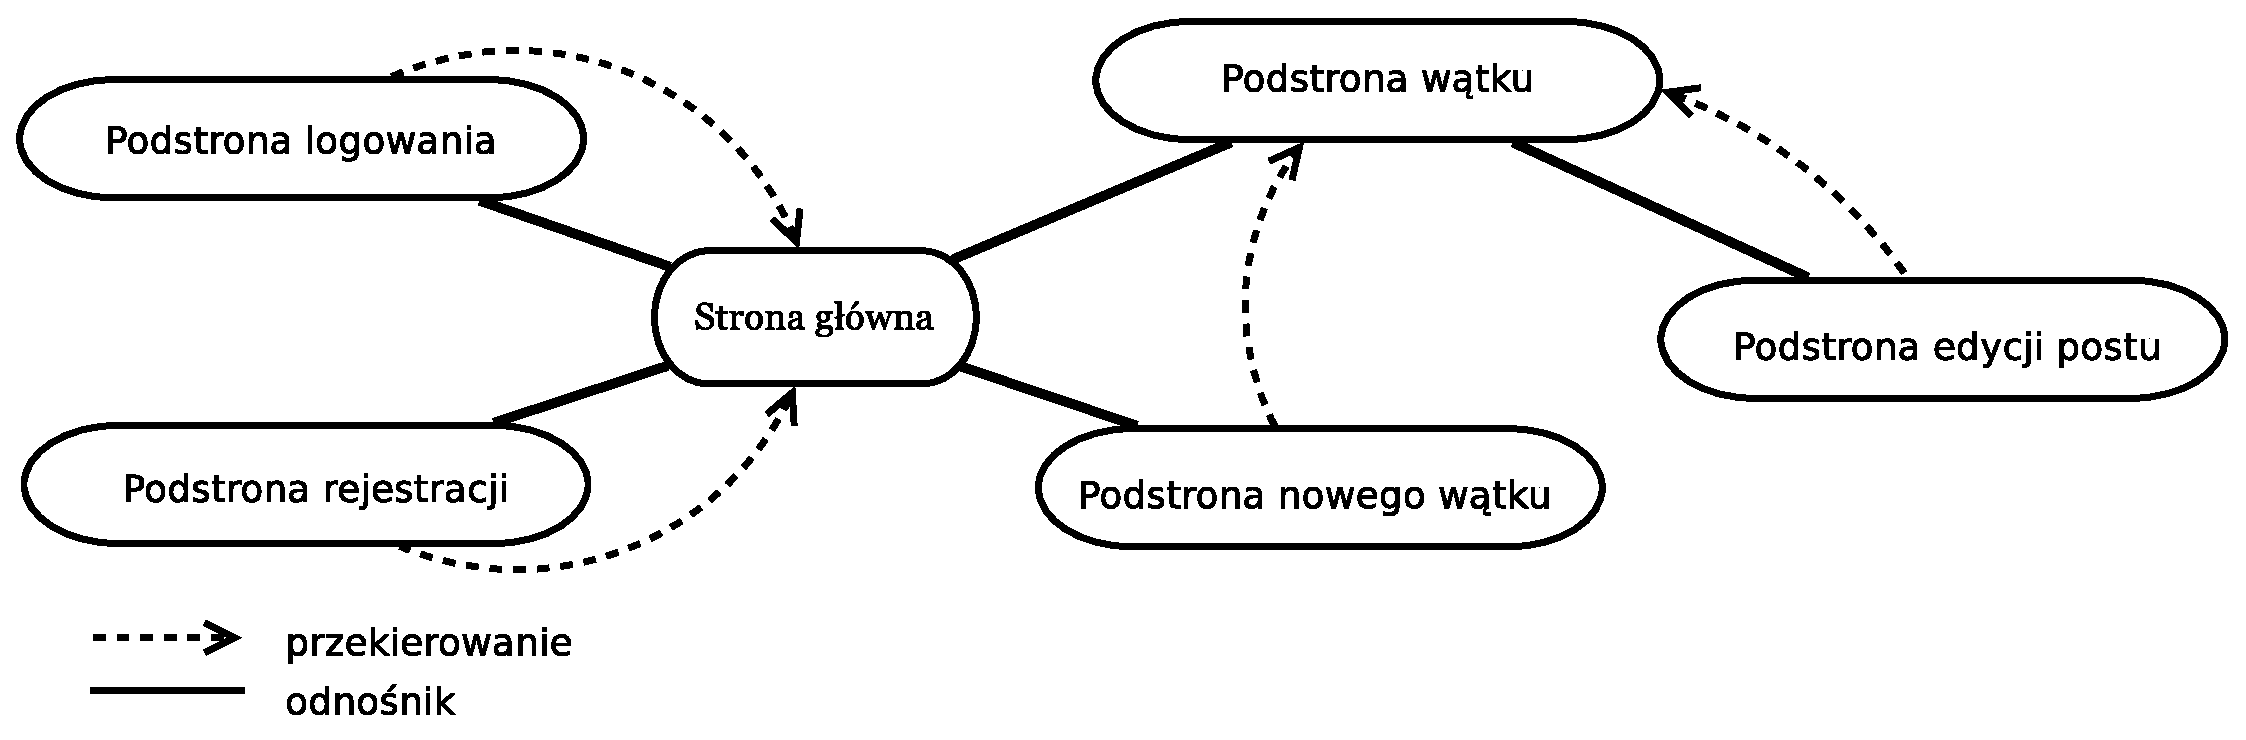
\includegraphics[width=0.9\textwidth]{subp.eps}
\caption{Układ podstron forum}
\end{figure}


\subsection{Projekt bazy danych}
Informacje w bazie danych są przechowywane w postaci tabel, podobnie jak w arkuszach kalkulacyjnych dostępnych w popularnych pakietach biurowych. W bazie projektowanego forum będziemy przechowywać listę użytkowników, listę tematów oraz listę postów. Dla każdej z tych list trzeba utworzyć oddzielną tabelę: users, threads, posts. W każdej z tych tabel konieczne jest stworzenie odpowiednich kolumn służących do przechowywania danych we właściwych typach. Ustawienie typu danej przechowywanej w każdej kolumnie przyśpiesza pracę serwera MySQL poprzez automatyczną optymalizację realizowanych zapytań do bazy oraz optymalizację sposobu przechowywania tabel na dysku.
\subsubsection{Typy danych MySQL}
W języku MySQL jest wiele typów danych 
(dokładny opis: \href{http://dev.mysql.com/doc/refman/5.5/en/data-type-overview.html}{http://dev.mysql.com/doc/refman/5.5/en/data-type-overview.html}), te najważniejsze to:

\paragraph{Typy znakowe:}
\begin{description}[5mm]
\item[CHAR] Przechowuje ciąg znaków do 255 elementów.
\item[VARCHAR] Tak jak \textbf{CHAR} przechowuje ciąg znaków do 255 elementów. Główną różnicą pomiędzy nimi jest to, że \textbf{VARCHAR} zmienia swój rozmiar w zależności od przyjętej liczby znaków, a \textbf{CHAR} zawsze rezerwuje miejsce 255 znaków niezależnie od długości zapisywanego ciągu.
\item[TEXT] Przechowuje ciąg do 65535 znaków.
\item[MEDIUMTEXT] Przechowuje ciąg do 16777215 znaków.
\end{description}

\paragraph{Typy liczbowe:}
\begin{description}[5mm]
\item[TINYINY] Przechowuje liczby od -128 do 127 (0 do 255 w przypadku \textbf{UNSIGNED}).
\item[SMALLINT] Przechowuje liczby od -32768 to 32767 (0 do 65535 w przypadku \textbf{UNSIGNED}).
\item[MEDIUMINT] Przechowuje liczby od -8388608 do 8388607 (0 do 16777215 w przypadku \textbf{UNSIGNED}).
\item[FLOAT] Małe liczby zmiennoprzecinkowe.
\item[DOUBLE] Liczby zmiennoprzecinkowe o podwojonej precyzji.
\end{description}
Każdy typ liczbowy występuje także w wersji \textbf{UNSIGNED}, która pozwala przechowywać dwa razy większe liczby bez przechowywania informacji o znaku.
\paragraph{Inne typy:}
\begin{description}[5mm]
\item[DATE] Data w formacie YYYY-MM-DD
\item[DATETIME] Data w formacie YYYY-MM-DD HH:MM:SS
\item[TIMESTAMP] Znacznik czasu w formacie: YYYYMMDDHHMMSS
\item[TIME] Czas w formacie: HH:MM:SS
\item[ENUM] Podobnie jak w C++, definiuje listę określonych wartości jakie może przyjąć to pole.
\item[SET] Podobnie jak \textbf{ENUM}, lecz pole w tabeli może przyjąć kilka wartości na raz.
\end{description}

\subsubsection{Projekty tabel}
Tabela \textit{users} powinna zawierać kolumny przechowujące informacje o użytkowniku takie jak: nazwa użytkownika, login używany przy identyfikacji na stronie, hash SHA-1\footnote{W bazach danych \textbf{NIGDY} nie powinno się przechowywać haseł w jawnej postaci tekstu. W przypadku gdy osoba trzecia uzyska nieautoryzowany dostęp do bazy danych, będzie mogła skopiować listę haseł wszystkich użytkowników, co nie powinno mieć nigdy miejsca. Zamiast tego przechowuje się specjalne hashe wygenerowane na podstawie haseł. Więcej informacji na temat hashy: \href{http://pl.wikipedia.org/wiki/Funkcja_skrótu}{pl.wikipedia.org}} hasła oraz pole determinujące czy dany użytkownik ma uprawnienia administracyjne (wartość 1, gdy użytkownik jest administratorem). \\
Tabela \textit{threads} powinna zawierać kolumny przechowujące tytuł wątku, zawartość pierwszego posta oraz data utworzenia wątku. \\
Tabela \textit{posts} powinna zawierać kolumny przechowujące treść posta i datę jego utworzenia. \\
Dodatkowo w każdej z tabel powinna znajdować się kolumna \textit{id} identyfikująca w każdej tabeli pojedynczy rekord. To rozwiązania ułatwia odwoływanie się do poszczególnych wpisów (rekordów)  w tabeli, bez konieczności ponownego przeszukiwania całej tabeli.
W tabelach \textit{posts} i  \textit{threads} oprócz informacji o postach i wątkach musimy utworzyć tak zwane relacje - kolumny wiążące poszczególne posty z użytkownikami oraz wątkami. Jest to tak zwana relacja \textbf{jeden do wielu}. Zagadnienie to można rozwiązać w prosty sposób: w tabeli \textit{threads} tworzymy kolumnę \textit{author\_id}, którą będzie zawierała id rekordu w tabeli \textit{users} odpowiadającego użytkownikowi, który stworzył dany wątek. Analogiczną operację trzeba wykonać dla tabeli posts: tworzymy kolumnę \textit{author\_id} oraz dodatkową \textit{thread\_id}, która definiuje wątek do którego przynależy dany post.

\begin{figure}[htbp]
\centering
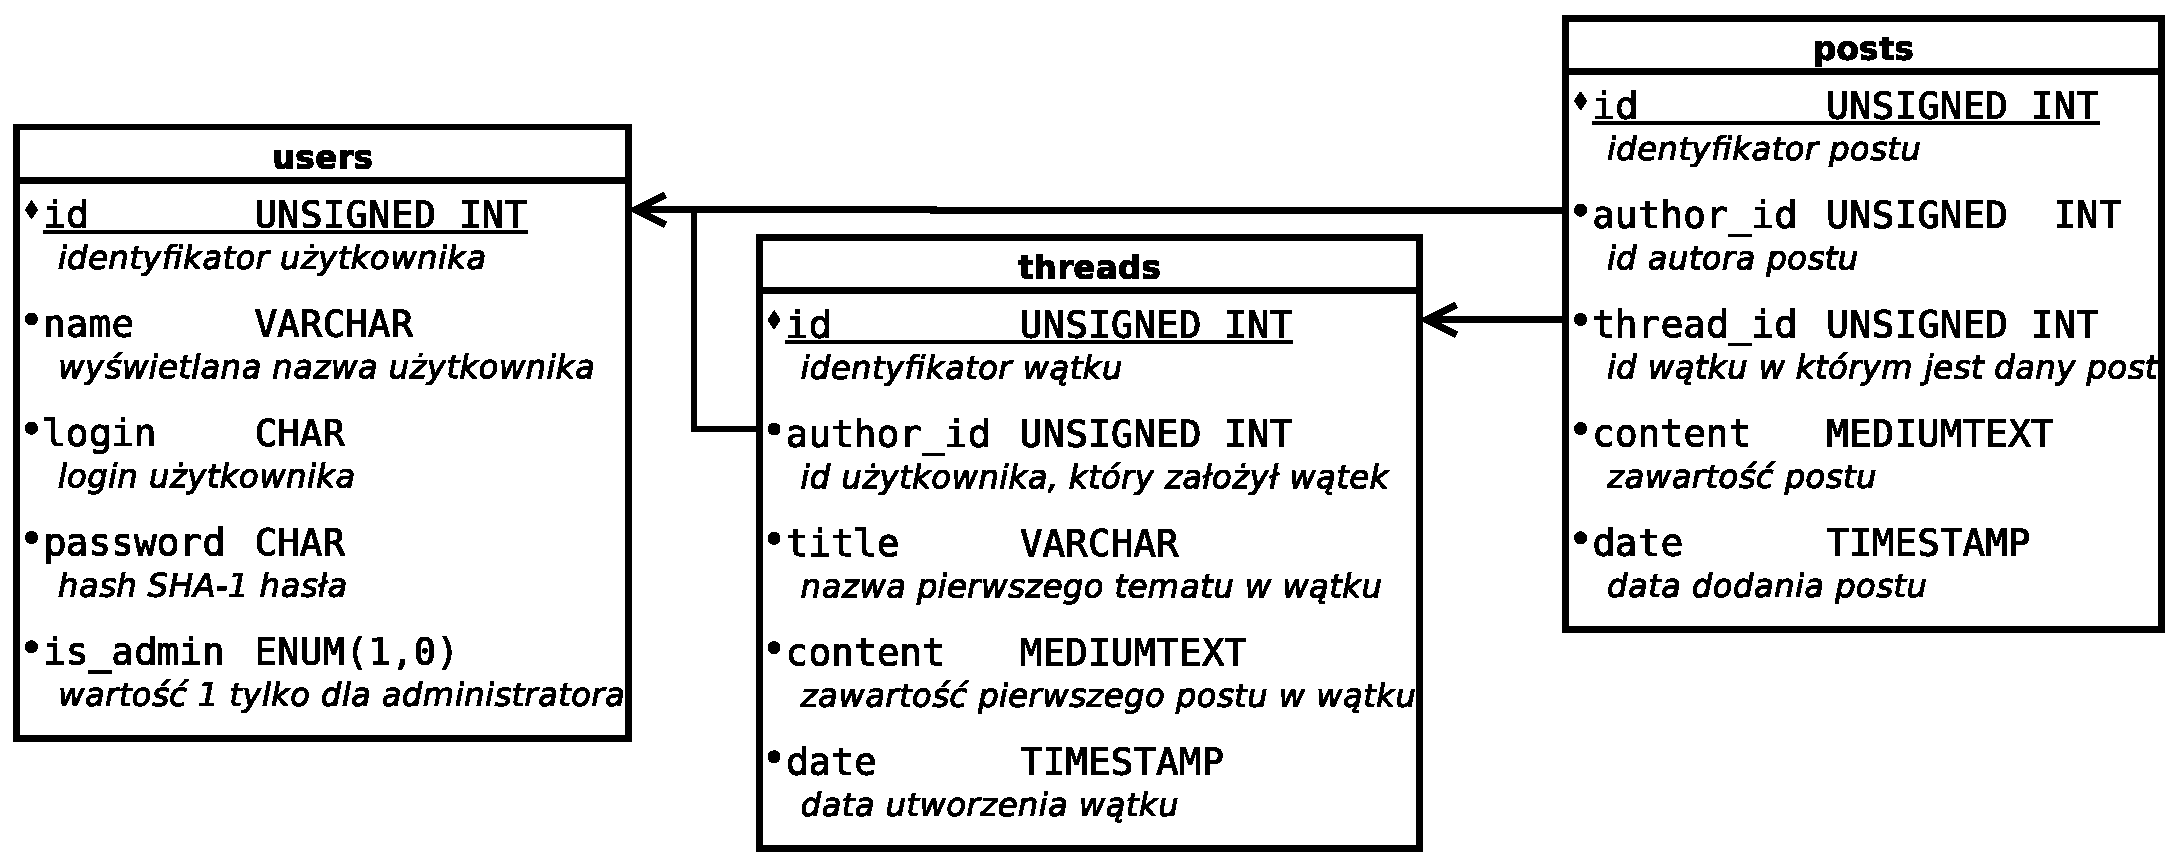
\includegraphics[width=1\textwidth]{db.eps}
\caption{Schematy tabel i ich wzajemne relacje}
\end{figure}

\paragraph{Optymalizacja}
Oprócz precyzowania typów danych dla każdej kolumny, aby ułatwić sobie i serwerowi pracę można zdefiniować dodatkowe atrybuty dla poszczególnych kolumn. Kolumna \textit{id} występująca w każdej z tabel musi być zdefiniowana z atrybutami \textit{PRIMARY KEY} (co jest zaznaczone na schemacie podkreśleniem) - oznacza to, że kolumna jest wykorzystywana do identyfikacji rekordów w tabeli, \textit{AUTO\_INCREMENT} - każdy dodawany rekord ma ustawiane automatycznie \textit{id} o 1 większe niż największe \textit{id} w tabeli, \textit{NOT NULL} - nie może mieć wartości 0.

\subsubsection{Kod SQL}
Nadszedł czas na stworzenie zaprojektowanej przez nas struktury tabel. Uruchamiamy serwer MySQL, a następnie poleceniem (dla systemu Linux): \\
\begin{minted}[bgcolor=code]{bash}
mysql -u root -p
\end{minted}
uruchamiamy wiersz poleceń MySQL.
Na systemie Windows aby uruchomić wiersz poleceń, wpierw trzeba uruchomić terminal, a w nim wpisać:  \\
\begin{minted}[bgcolor=code]{bat}
C:> cd C:\sciezka\do\katalogu\mysql\bin
C:\sciezka\do\katalogu\mysql\bin> mysql.exe -u root -p
\end{minted}
Następnie po wpisaniu hasła, aby stworzyć bazę danych wydajemy polecenie: \\
\begin{minted}[bgcolor=code]{sql}
CREATE DATABASE forum;
\end{minted}
Aby przystąpić do tworzenia tabel, trzeba wybrać nowo utworzoną bazę danych: \\
\begin{minted}[bgcolor=code]{sql}
USE forum;
\end{minted}
Możemy teraz utworzyć tabelę \textit{users} wydając poniższe polecenie: \\
\begin{minted}[linenos=true, bgcolor=code]{sql}
CREATE TABLE `forum`.`users` (
	`id` INT UNSIGNED NOT NULL AUTO_INCREMENT PRIMARY KEY ,
	`name` VARCHAR( 255 ) NOT NULL ,
	`login` CHAR( 255 ) NOT NULL ,
	`password` CHAR( 255 ) NOT NULL ,
	`is_admin` ENUM( '1', '0' ) NOT NULL ,
	UNIQUE (
		`name` ,
		`login` 
	)
);
\end{minted}
Ważne jest umieszczenie na końcu wyrażenia średnika, ponieważ informuje to interpreter MySQL że to jest koniec komendy. Bez średnika interpreter będzie czekał na dalsze wprowadzanie komend, dopóki nie napotka średnika.
W linii 1 podajemy nazwę bazy danych, a po kropce jest nazwa tworzonej tabeli. Nazwy bazy, tabel i kolumn są wzięte w ` `. W liniach 2-6 zdefiniowane są kolumny tabeli oddzielone przecinkami. Składnia jest następująca: \\
\begin{minted}[bgcolor=code]{sql}
`nazwa_kolumny` TYP NULL [dodatkowe atrybuty] ,
\end{minted}
Na początku podajemy nazwę kolumny, potem nazwę typu, jeżeli jest to typ liczbowy bez znaku, za nazwą typu dodajemy \textit{UNSIGNED}. Jeżeli jest to typ znakowy \textit{CHAR} lub \textit{VARCHAR} to wpisujemy w nawiasie maksymalną długość ciągu znaków. Jeżeli jest to typ \textit{ENUM}, lub \textit{SET} w nawiasie podajemy dopuszczalne wartości. Następnie podajemy informację czy w tą kolumnę może zostać wpisana wartość pusta - parametr \textit{NULL}, lub gdy nie: \textit{NOT NULL}. Jeżeli chcemy ustawić dodatkowe opcje dla kolumny wpisujemy je oddzielając spacją. Dla kolumny \textit{id} zostały ustawione opcje \textit{AUTO\_INCREMENT} oraz \textit{PRIMARY KEY}. Po wymienionych kolumnach można zdefiniować dodatkowe indeksy, w linii 7 zdefiniowany jest indeks \textit{UNIQUE}: dla kolumn umieszczonych w nawiasie wartości w pól w rekordach nie mogą się powtarzać. \\
Tabela \textit{threads}: \\
\begin{minted}[linenos=true, bgcolor=code]{sql}
CREATE TABLE `forum`.`threads` (
	`id` INT UNSIGNED NOT NULL AUTO_INCREMENT PRIMARY KEY ,
	`author_id` INT UNSIGNED NOT NULL ,
	`title` VARCHAR( 255 ) NOT NULL ,
	`content` MEDIUMTEXT NOT NULL ,
	`date` TIMESTAMP ON UPDATE CURRENT_TIMESTAMP NOT NULL DEFAULT CURRENT_TIMESTAMP 
);
\end{minted}
Kod jest prawie identyczny jak w poprzednim przypadku. Różnica pojawia się jedynie w linii 6. Po typie danych \textit{TIMESTAMP} zdefiniowana jest opcja \textit{ON UPDATE CURRENT\_TIMESTAMP}, która mówi, że po aktualizacji rekordu silnik bazy danych automatycznie umieści w kolumnie \textit{date} aktualny znacznik czasu. Następnie jest podana informacja, że wartość pola nie może być wartością \textit{NULL}. Parametr \textit{DEFAULT CURRENT\_TIMESTAMP} mówi nam, że gdy przy wpisywaniu wartości do bazy danych nie podamy wartości tego pola, serwer MySQL automatycznie wypełni to pole aktualną godziną. \\
Tabela \textit{posts}: \\
\begin{minted}[linenos=true, bgcolor=code]{sql}
CREATE TABLE `forum`.`posts` (
`id` INT UNSIGNED NOT NULL AUTO_INCREMENT PRIMARY KEY ,
`author_id` INT UNSIGNED NOT NULL ,
`thread_id` INT UNSIGNED NOT NULL ,
`content` MEDIUMTEXT NOT NULL ,
`date` TIMESTAMP ON UPDATE CURRENT_TIMESTAMP NOT NULL DEFAULT CURRENT_TIMESTAMP 
);
\end{minted}
Składnia jest analogiczna jak w poprzednim wypadku. Powyższe trzy zapytania \textit{CREATE} tworzą już kompletną, ale jeszcze pustą strukturę naszej bazy danych.
\section{Kod strony}
Przed przystąpieniem do pracy nad kodem strony, warto wyposażyć się w jakikolwiek edytor z kolorowaniem składni. Na systemy z rodziny Windows dobrym rozwiązaniem jest Notepad++, dostępny ze strony: \href{http://notepad-plus-plus.org/download/v6.1.2.html}{http://notepad-plus-plus.org/download/v6.1.2.html}. Na systemach GNU (w tym tych z rodziny Linux) może to być Emacs, Vim, Nano lub używany w środowisku Gnome, Gedit.
\subsection{Składnia języka PHP}
Przykładowy kod strony w języku php: \\
\begin{minted}[linenos=true, bgcolor=code]{php}
<?php
$jeden = 'bar';
$dwa = "foo";
$trzy = null;
$liczba = "4";
$liczba2 = 3;
if($liczba % 2 == 0)
{
	echo 'liczba jest podzielna przez 2 <br />';
}
else
{
	echo 'liczba nie jest podzielna przez 2 <br />';
}

if($liczba == 4)
	echo 'Ta liczba to 4!';
elseif($liczba < 4)
	echo 'Ta liczba jest mniejsza od 4.<br />';
else
	echo 'Ta liczba jest wieksza od 4 <br />';
echo $jeden.$dwa.($liczba+$liczba2);
?>
\end{minted}
Zapisując powyższy kod jako plik \textit{index.php} w katalogu /var/www (lub c:/etc/www/ na systemie Windows), a następnie wchodząc na stronę http://127.0.0.1/ otrzymamy wynik:
\begin{minted}{php}
liczba jest podzielna przez 2
Ta liczba to 4!
barfoo7
\end{minted}
Kod PHP aby został wykonany musi być zawarty w tagach \textit{<?php ?>}.
W linijkach 2 - 6 zostały zdefiniowane zmienne. Nazwy zmiennych muszą być poprzedzone znakiem \$ zarówno przy definiowaniu jak i późniejszym odwoływaniu się do nich. Ciąg znaków przypisywany do zmiennej można zawszeć w apostrofach lub cudzysłowach. Między tymi dwoma sposobami jest niewielka różnica: gdy zawrzemy ciąg znaków w cudzysłowach PHP przeszukuje zawartość ciągu pod kątem znaków specjalnych (np.: \textbackslash n \textbackslash r itp.), w przypadku apostrofów przeszukiwanie nie jest dokonywane (ta forma jest nieco szybsza). W liniach 7 - 21 są umieszczone struktury \textit{if - else}. W linii 7 jest wykonywane modulo na zmiennej \textit{\$liczba}, a następnie wynik tej operacji jest przyrównywany do zera. Należy zwrócić uwagę iż w PHP brak jest typów zmiennych - zależnie od potrzeb zmienna jest automatycznie traktowana jako ciąg znaków, lub jako liczba. W linii 9 do wyświetlania jest używana struktura języka: \textit{echo}. W linii 22 został użyty operator konkatenacji (kropka) do połączenia trzech ciągów znaków w jeden. Najpierw zostało wykonane dodawanie dwóch liczb w nawiasie, a następnie ich suma została zamieniona na ciąg znaków, który został doklejony do fraz 'bar' i 'foo'. W PHP operator kropki nie jest używany w odniesieniu do obiektów (jak to ma miejsce w Javie i w C++).
\pagebreak
Przykładowa klasa w PHP: \\
\begin{minted}[linenos=true, bgcolor=code]{php}
<?php
class Telewizor
{
	private static $iloscTelewizorow = 0;
	
	private $aktualnyKanal = 0;
	private $poziomGlosnosci = 50;
	
	public static function pobierzLiczbeTelewizorow()
	{
		return self::$iloscTelewizorow;
	}
	
	public function __construct()
	{
		++self::$iloscTelewizorow;
	}
	
	public function ustawGlosnosc($poziomGlosnosci)
	{
		$this->poziomGlosnosci = $poziomGlosnosci;
	}
	
	public function ustawKanal($nrKanalu = 0)
	{
		$this->aktualnyKanal = $nrKanalu;
	}
};

function wyswietlaj()
{
	echo 'teraz wyswietlaja '.Telewizor::pobierzLiczbeTelewizorow().' telewizory';
}

new Telewizor;
new Telewizor;
$sharp =  new Telewizor;
$sharp->ustawKanal();
$sharp->ustawKanal(13);
$sharp->ustawGlosnosc(30);
$sharp->ustawGlosnosc(10);

wyswietlaj();
?>
\end{minted}
Wynik:
\begin{minted}{php}
teraz wyswietlaja 3 telewizory
\end{minted}
Składnia jest bardzo podobna do tej znanej z C++, za wyjątkiem braków typów zmiennych. W liniach 4 - 7 zostały zadeklarowane i zainicjalizowane domyślnymi wartościami właściwości klasy. W linii 11 jest odwołanie do statycznej właściwości klasy. W PHP dostęp do statycznych pól klasy jest uzyskiwany za pomocą wyrażenia self i operatora dostępu "::". W linii 14 znajduje się konstruktor, którego zadaniem jest zwiększanie ilości stworzonych telewizorów. W PHP konstruktory i destruktory noszą zawsze nazwę \textit{\_\_construct()} i \textit{\_\_destruct()} niezależnie od nazwy klasy. W deklaracji każdej funkcji i metody zawsze znajduje się słowo kluczowe function. W linii 21 jest ustawiany poziom głośności w telewizorze. Dostęp do właściwości obiektów uzyskać można tylko za pomocą wskaźnika \textit{\$this} wskazującego na aktualny obiekt, dostępnego w każdej \textbf{niestatycznej} metodzie klasy. Należy zwrócić uwagę, że gdy odwołujemy się do właściwości klasy za pomocą \textit{\$this} nie używamy już \textit{\$} przed nazwą pola klasy. W linii 24 została zdefiniowana funkcja przyjmująca parametr, który ma już wartość domyślną. Jest to pewien odpowiednik znanego z C++ przeciążania funkcji, gdy kilka funkcji mogło mieć tą samą nazwę - różnił je tylko zestaw argumentów. W PHP przeciążanie funkcji znane z C++ jest niedozwolone, zamiast tego stosuje się wartości domyślne argumentów. Pozwala to na wywołanie funkcji bez podawania argumentów, którym zostały przypisane wartości domyślne w nagłówku funkcji. Przykład takiego wywołania jest w linii 38 i 39.
Obiekty tworzy się za pomocą operatora \textit{new}, przykład znajduje się w liniach 35 - 37. W liniach 35 i 36 tworzone są obiekty klasy Telewizor, które nie są do niczego przypisywane. W linii 37 tworzony obiekt tej samej klasy przypisany do zmiennej \textit{\$sharp}. Dostęp do pól i metod uzyskiwany jest za pomocą operatora -> .
\paragraph{Zagnieżdżanie wewnątrz kodu HTML} PHP umożliwia przeplatanie kodu HTML i PHP, co umożliwia generowanie zawartości stron w czasie rzeczywistym. Przykład kodu: \\
\begin{minted}[linenos=true, bgcolor=code]{php}
<!DOCTYPE HTML>
<html>
<head>
 <title>Forum</title>
 <meta charset="UTF-8" />
</head>
<body>
<?php if(!is_object(User::$oCurrentUser)):?>
<a href="register.php">rejestracja</a>
<?php else: ?>
Witaj <b><?php echo User::$oCurrentUser->sName; ?></b>
<?php endif; ?>
<br /><br />
<?php if(count($aThreads) > 0):?>
Lista watkow na forum:
<table border="1">
<?php foreach($aThreads as $i => $oThread): ?>
<tr>
 <td><?php echo $i+1 ?></td>
 <td>
<a href="thread.php?id=<?php echo $oThread->iId ?>">
<?php echo $oThread->sTitle ?></a>
<?php 
 if(is_object(User::$oCurrentUser))
	 if(User::$oCurrentUser->bIsAdmin)
	 	echo ' <a href="delete.php?tid='.$oThread->iId.'">[ usun ]</a>'; 
?></td>
 <td><?php echo $oThread->sAuthorName ?></td>
 <td><?php echo $oThread->sDate ?></td>
</tr>
<?php endforeach?>
</table>
<?php else: ?>
Brak watkow na forum.
<?php endif;?>
</body>
</html>
\end{minted}
W linii 8 jest wstawiona funkcja \textit{if()}. Należy zwrócić uwagę na dwukropek postawiony za nawiasem - w tym wypadku cała zawartość aż do linii 10, w której występuje \textit{else:} jest wyświetlana gdy warunek jest spełniony\footnote{dokładnie: gdy statyczne pole klasy \textit{User::\$oCurrentUser} nie jest obiektem - służy do tego funkcja \textit{\href{http://www.php.net/manual/en/function.is-object.php}{is\_object()}}}. Koniec \textit{if()} jest w linii 12. W linii 11 wyświetlane jest pole \textit{sName} zmiennej \textit{User::\$oCurrentUser} za pomocą wyrażenia \textit{echo}. W linii 17 występuje wyrażenie \textit{foreach()}. Ten zapis należy zrozumieć jako: dla każdego elementu tablicy \textit{\$aThreads} wykonaj pętlę, ale na początku pętli przypisz ten element na którym będziemy operować do zmiennej \$oThread, a klucz pod jakim ten element znajdował się w tablicy \$aThreads do zmiennej \textit{\$i}. W przypadku zwykłych tablic, w których jest po prostu lista elementów, w zmiennej \textit{\$i} będzie znajdować się numer elementu w tablicy (w PHP tablice są numerowane od 0, tak jak w C/C++), a gdy \textit{\$aThreads} będzie tablicą asocjacyjną (taką, w której kluczami są ciągi znaków) \textit{\$i} będzie zawierało ciąg znaków, który był kluczem dla wartości \textit{\$oThread}. Koniec pętli \textit{foreach()} jest w linii 31.\\ Szczegółowe informacje na temat budowy języka można znaleźć w podręczniku PHP: \\ \href{http://www.php.net/manual/pl/langref.php}{http://www.php.net/manual/pl/langref.php}.
\subsection{Struktura plików forum}
Kod tworzonego forum będzie pogrupowany w następujące pliki:
\begin{description}[5mm]
\item[dao/Thread.php] Klasa reprezentująca pojedynczy wątek. Umożliwia tworzenie nowego wątku, modyfikację i listowanie wszystkich odpowiedzi.
\item[dao/Post.php] Klasa reprezentująca pojedynczą odpowiedź na wątek. Umożliwia tworzenie i modyfikację poszczególnych postów.
\item[dao/User.php] Klasa reprezentująca użytkownika - używana do zarządzania i identyfikacji użytkowników forum.
\item[add.php] Podstrona odpowiedzialna za dodawanie nowego wątku.
\item[init.php] Plik załączany w każdej podstronie odpowiedzialny za tworzenie połączenia z bazą danych i za dołączenie wymaganych plików.
\item[index.php] Strona główna forum. Wyświetla listę wątków na forum.
\item[delete.php] Podstrona odpowiedzialna za usuwanie wątków i odpowiedzi na forum.
\item[register.php] Podstrona rejestracji nowego użytkownika.
\item[config.php] Plik zawierający dane do połączenia z bazą danych.
\item[edit.php] Podstrona edycji wątku i postu.
\item[login.php] Podstrona odpowiedzialna za logowanie się użytkownika na forum.
\item[thread.php] Podstrona wyświetlająca zawartość całego wątku.
\end{description}
Nazwa folderu dao jest skrótem od Data Access Object. Zawiera on Klasy udostępniające warstwę abstrakcji pomiędzy kodem strony a bazą danych. Wszystkie pliki muszą zostać umieszczone w folderze /var/www (lub C:/etc/www na systemie Windows).
\subsection{Zawartość poszczególnych plików}
Na początek stwórzmy zawartość katalogu \textit{dao/} - obiekty umożliwiające dostęp do bazy danych.
%TODO POPRAWIĆ WSZYSTKIE WSTAWKI MINTED
\subsubsection{dao/Post.php}
Klasa umożliwiająca zarządzanie odpowiedziami, będzie zawierać metody \textit{save()} oraz \textit{delete()}, które będą odpowiedzialne za zapisywanie posta do bazy (a także modyfikowanie już istniejącego). W poniższych listingach została przyjęta konwencja poprzedzania nazw zmiennych literą reprezentującą umowny typ wartości jaki będzie w danej zmiennej przechowywany. Odpowiednio i - integer, s - string, a - array, b - bool.
\paragraph{Wskazówka:} W trakcie pisania kodu, gdy nasza zaprojektowana aplikacja nie będzie działać jak powinna, można podczas debuggowania kodu wspomóc się funkcją  \textit{var\_dump()}\footnote{\href{http://www.php.net/manual/en/function.var-dump.php}{http://www.php.net/manual/en/function.var-dump.php}}.
\\
\begin{minted}[linenos=true, bgcolor=code]{php}
<?php
class Post
{
	static public $oConnection = null;

	public $iId = null;
	public $iAuthorId = null;
	public $sAuthorName = null;
	public $iThreadId = null;
	public $sContent = null;
	public $sDate = null;
	
	public function __construct($iId = null){}
	
	public function save(){}

	public function delete(){}
};
?>
\end{minted}
W linii 4 zdefiniowane jest statyczne pole \textit{\$oConnection}, które będzie reprezentować obiekt klasy PDO (dostarczonej wraz z PHP). Klasa PDO jest używana do komunikacji z bazą danych. W każdej z klas Post, Thread, User zostało umieszczone statyczne pole, które będzie przechowywało referencję do obiektu klasy PDO, aby móc się komunikować z bazą danych. \\
W liniach 6-11 są umieszczone pola reprezentujące odpowiednie kolumny w bazie danych, odpowiednio kolumny id, author\_id, thread\_id, content, date. Dodatkowo została zadeklarowane pole \textit{\$sAuthorName}, która będzie przechowywała nazwę autora postu. W linii 13 został zadeklarowany konstruktor przyjmujący domyślnie wartość \textit{null}. Gdy będzie tworzony nowy post, do konstruktora nie trzeba podawać żadnego parametru. W przypadku gdy będzie potrzeba stworzenia obiektu reprezentującego już istniejący post, zmienna \textit{\$iId} będzie reprezentowała id odpowiedniego rekordu już istniejącego w bazie. \\
Zawartość metody \textbf{\_\_construct()} (która znajduje się pomiędzy klamrami w wyżej wymienionym listingu): \\
\begin{minted}[linenos=true, bgcolor=code]{php}
<?php
public function __construct($iId = null)
{
	$this->iId = $iId;
	if($iId != null)
	{
		$oStatement = self::$oConnection->prepare('
				SELECT *,`posts`.`id` AS `pid` 
				FROM `posts`,`users`
				WHERE `posts`.`author_id`=`users`.`id`
				AND `posts`.`id` = :id
				ORDER BY `posts`.`id` ASC');
		$oStatement->bindValue(':id', $iId, PDO::PARAM_INT);
		$oStatement->execute();
		if($oStatement->errorCode() != 0)
		{
			$aError = $oStatement->errorInfo();
			throw new Exception($aError[2]);
		}
\end{minted}
\begin{minted}[linenos=true, bgcolor=code,firstnumber=15]{php}
		if($aResult = $oStatement->fetch(PDO::FETCH_ASSOC))
		{
			$this->iId = $aResult['pid'];
			$this->iAuthorId = $aResult['author_id'];
			$this->sAuthorName = $aResult['name'];
			$this->iThreadId = $aResult['thread_id'];
			$this->sContent = $aResult['content'];
			$this->sDate = $aResult['date'];
		}
		else
			$this->iId = null;
	}
}
?>
\end{minted}
W linii 5, jeżeli zostało podane id postu rozpoczyna się procedura odczytu z bazy danych. W pierwszym kroku konieczne jest utworzenie szkieletu zapytania za pomocą metody \textit{prepare()}, do której jako parametr przekazujemy zapytanie. Aby wyciągnąć dane z bazy trzeba użyć zapytania \textit{SELECT}, którego składnia jest następująca:\\
\begin{minted}[bgcolor=code]{sql}
SELECT `kolumna1`,`kolumna2`,`kolumna3` FROM `tabela`;
\end{minted}
Oznacza to, że pobieramy dane z kolumn: `kolumna1`, `kolumna2` i `kolumna3` z tabeli `tabela`. Zamiast listy kolumn można także podać gwiazdkę *, która oznacza, że wybieramy z tabeli wszystkie kolumny. Można w jednym zapytaniu \textit{SELECT} pobierać dane z kilku tabel na raz - trzeba wtedy je wymienić po klauzuli \textit{FROM} oddzielając je przecinkami. Gdy odwołujemy się do kilku tabel na raz, należy pamiętać o poprzedzeniu nazw kolumn nazwą tabeli. Zapytanie SQL wyglądałoby w ten sposób: \\
\begin{minted}[bgcolor=code]{sql}
SELECT `tabela`.`kolumna1`,`tabela`.`kolumna2`,`tabela`.`kolumna3`,`tabela2`.`kolumna5`
FROM `tabela`,`tabela2`;
\end{minted}
Kolejny przykład: \\
\begin{minted}[bgcolor=code]{sql}
SELECT `kolumna1`,`kolumna2`,`kolumna3`
FROM `tabela`
WHERE `kolumna1` = `kolumna2`
ORDER BY `kolumna1` ASC;
\end{minted}
Powyższe zapytanie zwraca tylko te rekordy z tabeli `tabela`, w których wartości w kolumnie `kolumna1` są identyczne jak w `kolumna`. Jak widać słowo kluczowe \textit{WHERE} służy do tworzenia warunków, jakie muszą spełniać zwrócone rekordy. Warunki w części zapytania po \textit{WHERE} mogą być łączone za pomocą operatorów \textit{OR} oraz \textit{AND}. Wiersz który zawiera frazę \textit{ORDER BY} mówi serwerowi MySQL, żeby zwrócone wyniki zostały posortowane według zawartości kolumny `kolumna1` rosnąco (wyraz \textit{ASC} - ascending). Można także posortować wyniki malejąco: \textit{DESC} - descending. Fragmenty zapytania z \textit{WHERE} oraz \textit{ORDER BY} są opcjonalne. W zapytaniu można dodatkowo przypisać zwracanym kolumnom nową nazwę - służy do tego słowo klucz \textit{AS}: \\
\begin{minted}[bgcolor=code]{sql}
SELECT `kolumna1`,`kolumna2` AS `ilosc`,`kolumna3`
FROM `tabela`
WHERE `kolumna1` = `kolumna2`
ORDER BY `kolumna1` ASC;
\end{minted}
W powyższym zapytaniu, zwrócony wynik będzie zawierał kolumnę `kolumna2` nazwaną jako `ilosc`. \\
Wracając do zapytania przekazanego jako argument do metody \textit{prepare()}\footnote{\href{http://www.php.net/manual/en/pdo.prepare.php}{http://www.php.net/manual/en/pdo.prepare.php}}, wybieramy za pomocą niego wszystkie kolumny z tabel `posts` i `users`, nazywając kolumnę `id` w tabeli `posts` jako `pid`, a następnie pobieramy rekordy z obydwu tabel, dla których id postu odpowiada id użytkownika w tabeli `users` (klauzula \textit{WHERE}: `posts`.`author\_id`=`users`.`id` ) oraz id postu jest równe numerowi id przez nas poszukiwanemu. Na koniec zwrócone dane są posortowane względem id postu. To zapytanie powinno zwrócić jeden wynik (ponieważ, kolumna `id` jest kluczem głównym w tabeli `posts`) - post przez nas poszukiwany, dodatkowo wraz z nazwą autora postu w kolumnie `name`. W zapytaniu nie zostało wpisane id przez nas poszukiwane - zamiast tego został umieszczony tag \textit{:id}, który za pomocą funkcji \textit{bindValue()}\footnote{\href{http://www.php.net/manual/en/pdostatement.bindvalue.php}{http://www.php.net/manual/en/pdostatement.bindvalue.php}} jest zastępowany wartością id postu. To rozwiązanie ma na celu oczyszczenie danych wejściowych z niebezpiecznych znaków, które mogłyby zepsuć składnię zapytania i uniemożliwić jego poprawne wykonanie (a poprzez celową manipulację możliwe by było nawet skasowanie zawartości bazy\footnote{\href{http://pl.wikipedia.org/wiki/SQL_injection}{http://pl.wikipedia.org/wiki/SQL\_injection}}). Drugi argument metody \textit{bindValue()} mówi jakiego typu zmienna jest przekazywana. Metoda \textit{prepare()} zwraca obiekt typu \textit{PDOStatement} reprezentujący zapytanie które jest wysyłane do bazy danych. \\
W linii 14 zapytanie jest wykonywane. W linii 15 jest sprawdzana poprawność wysłanego zapytania, gdy zapytanie zostanie wykonane niepoprawnie zostanie rzucony wyjątek w linii 18, który będzie zawierał informację o błędzie który wystąpił. Funkcja \textit{errorInfo()}\footnote{\href{http://www.php.net/manual/en/pdostatement.errorinfo.php}{http://www.php.net/manual/en/pdostatement.errorinfo.php}} zwraca dostępną informację o błędzie w formie tablicy. W trzecim elemencie (o indeksie 2) znajduje się informacja opisowa o błędzie, którą przekazujemy konstruktorowi klasy Exception. \\
W linii 20, gdy zapytanie zostało wykonane bez żadnego błędu zostaje przypisana do zmiennej \$aResult tablica asocjacyjna (decyduje o tym parametr \textit{PDO::FETCH\_ASSOC} przekazany do metody \textit{fetch()}\footnote{\href{http://www.php.net/manual/en/pdostatement.fetch.php}{http://www.php.net/manual/en/pdostatement.fetch.php}}). Jeżeli \textit{\$aResult} jest niepuste (co w PHP jest równoznaczne wartości true) zostanie spełniony warunek i w liniach 22-27 dane ze zwróconej tablicy asocjacyjnej są przypisywane odpowiednim właściwościom obiektu. Należy zwrócić uwagę, na to, że klucze w zwróconej tablicy odpowiadają kolumnom zdefiniowanym w zapytaniu. Jeżeli warunek z linii 20 nie zostanie spełniony, przypisujemy właściwości \textit{\$iId} wartość \textit{null}, która odpowiada operacji tworzenia nowego indeksu. Wartość pola \textit{\$iId} jest rozpoznawana w metodzie \textit{save()}. \\
Zawartość metody \textbf{save()}: \\
\begin{minted}[linenos=true, bgcolor=code]{php}
<?php
public function save()
{
	if($this->iId != null) // update
	{
		$oStatement = self::$oConnection->prepare('
			UPDATE `posts` 
			SET
				`author_id` = :aid,
				`thread_id` = :tid,
				`content` = :content 
			WHERE `id` =:id ');
		$oStatement->bindValue(':id', $this->iId, PDO::PARAM_INT);
	}
	else // insert
		$oStatement = self::$oConnection->prepare('
			INSERT INTO `posts` (`author_id` ,`thread_id` ,`content`) 
			VALUES (:aid, :tid, :content);');
	$oStatement->bindValue(':aid', $this->iAuthorId, PDO::PARAM_INT);
	$oStatement->bindValue(':tid', $this->iThreadId, PDO::PARAM_INT);
	$oStatement->bindValue(':content', $this->sContent, PDO::PARAM_STR);
	$oStatement->execute();
	if($oStatement->errorCode() != 0)
	{
		$aError = $oStatement->errorInfo();
		throw new Exception($aError[2]);
	}
	if($this->iId == null) 
		$this->iId = self::$oConnection->lastInsertId();
}
?>
\end{minted}
W linii 4 jest rozróżnienie czy wpisujemy nową wartość do bazy, czy też aktualizujemy istniejący już rekord.\\
W linii 6 jest przygotowywane zapytanie \textit{UPDATE} przed wykonaniem go. Składnia zapytania jest podobna do składni zapytania \textit{SELECT}. Po frazie \textit{UPDATE} podawana jest nazwa tabeli którą aktualizujemy, następnie po wyrazie \textit{SET} podawane są nowe wartości odpowiednich kolumn, rozdzielone przecinkami. Nie trzeba wymieniać wszystkich kolumn jakie są w tabeli - te niewymienione zachowają swoją niezmienioną wartość. Klauzula \textit{WHERE} w zapytaniu \textit{UPDATE} determinuje który rekord w bazie danych ma zostać zmodyfikowany. Jej składnia jest identyczna jak w przypadku zapytania \textit{SELECT}. Za pomocą zapytania \textit{UPDATE} można modyfikować jeden lub wiele rekordów w bazie danych na raz.\\
W linii 15 jest przygotowywane zapytanie wstawiające nową wartość do bazy danych. Po frazie \textit{INSERT INTO} jest wymieniona nazwa tabeli, a w nawiasie oddzielone przecinkami wartości kolumn. Ważne jest, że przy zapytaniu \textit{INSERT} należy wymienić wszystkie kolumny z tabeli, którym nadaliśmy atrybut \textit{NOT NULL} przy projektowaniu bazy danych. Po wyrażeniu \textit{VALUES} są podane wartości które zostaną wstawione do bazy danych. Wartości kolejno odpowiadają wcześniej wymienionym kolumnom i muszą być oddzielone przecinkami. W powyższych zapytaniach znowu użyliśmy fraz zastępczych :aid, :tid etc., które zostają potem dopiero podmienione za pomocą funkcji \textit{bindValue()}. \\
W linii 22 tak jak w poprzednim przypadku jest weryfikowana poprawność zapytania. \\
W linii 28 jeżeli był wykonywany \textit{INSERT} odzyskujemy wartość kolumny `id` za pomocą metody \linebreak \textit{lastInsertId()}\footnote{\href{http://www.php.net/manual/en/pdo.lastinsertid.php}{http://www.php.net/manual/en/pdo.lastinsertid.php}}, które umożliwi nam późniejsze odwoływanie się do umieszczonego w bazie postu.\\



Zawartość metody \textbf{delete()}: \\
\begin{minted}[linenos=true, bgcolor=code]{php}
<?php
public function delete()
{
	$oStatement = self::$oConnection->prepare('
		DELETE FROM `posts` WHERE `id` = :id');
	$oStatement->bindValue(':id', $this->iId, PDO::PARAM_INT);
	$oStatement->execute();
	if($oStatement->errorCode() != 0)
	{
		$aError = $oStatement->errorInfo();
		throw new Exception($aError[2]);
	}
	$this->iId = null;
}
?>
\end{minted}
W linii 5 jest przygotowywane zapytanie usuwające post z bazy danych. Po wyrażeniu \textit{DELETE FROM} podana jest nazwa tabeli z której usuwamy rekordy, a klauzula WHERE determinuje który rekord ma zostać usunięty.

\subsubsection{dao/Thread.php}
Klasa Thread pozwalająca na manipulację wątkami: \\
\begin{minted}[linenos=true, bgcolor=code]{php}
<?php
class Thread
{
	static public $oConnection = null;

	public $iId = null;
	public $iAuthorId = null;
	public $sAuthorName = null;
	public $sTitle = null;
	public $sContent = null;
	public $sDate = null;
	public $aPosts = array();

	static public function getAll() {}

	public function __construct($iId = null){}

	public function getAllPosts(){}

	public function getLastAnswer(){}

	public function save(){}

	public function delete(){}
};
?>
\end{minted}
W linii 4 jest zadeklarowane statyczne pole przechowujące obiekt reprezentujący połączenie z bazą danych. W liniach 6-12 są zadeklarowane właściwości klasy odpowiadające poszczególnym kolumnom w bazie danych. W linii 12 została zadeklarowana zmienna \textit{\$aPosts}, która będzie przechowywać wszystkie odpowiedzi w temacie reprezentowanym przez obiekt typu Thread. \\
Klasa zawiera statyczną metodę \textit{getAll()}, która pozwala na pobranie wszystkich wątków z bazy danych, metodę \textit{getAllPosts()}, która zwraca wszystkie odpowiedzi w temacie, metodę \textit{getLastAnswer()}, która pobiera ostatnią odpowiedź oraz metody \textit{save()} i \textit{delete()} pozwalające na zapisanie do bazy oraz na usunięcie wątku. Konstruktor podobnie jak w klasie Post, przyjmuje id poszukiwanego wątku, jeżeli nie zostanie nic podane przy wywołaniu konstruktora, zostanie utworzony nowy wątek.\\
Zawartość metody \textbf{getAll()}: \\
\begin{minted}[linenos=true, bgcolor=code]{php}
<?php
static public function getAll()
{
	$aThreads = array();
	$oStatement = self::$oConnection->prepare('
			SELECT *,`threads`.`id` AS `tid`
			FROM `threads`,`users`
			WHERE `threads`.`author_id`=`users`.`id`
			ORDER BY `threads`.`id` DESC');
	$oStatement->execute();
	if($oStatement->errorCode() != 0)
	{
		$aError = $oStatement->errorInfo();
		throw new Exception($aError[2]);
	}
\end{minted}
\begin{minted}[linenos=true, bgcolor=code,firstnumber=16]{php}
	while($aResult = $oStatement->fetch(PDO::FETCH_ASSOC))
	{
		$oThread = new self();
		$oThread->iId = $aResult['tid'];
		$oThread->iAuthorId = $aResult['author_id'];
		$oThread->sAuthorName = $aResult['name'];
		$oThread->sTitle = $aResult['title'];
		$oThread->sContent = $aResult['content'];
		$oThread->sDate = $aResult['date'];
		$aThreads[] = $oThread;
	}
	return $aThreads;
}
?>
\end{minted}
Budowa jest prawie identyczna jak jak w przypadku konstruktora klasy Post. W linii 4 deklarujemy zmienną \textit{\$aThreads}, która będzie przechowywała tablicę wszystkich wątków na forum. W następnych liniach przygotowujemy zapytanie \textit{SELECT}, pobierające listę wątków wraz z nazwami autorów z tablicy `users`, zostaje ono wykonane i jeżeli nie ma żadnego błędu to wchodzimy do pętli while. W warunku pętli while jest pobierany w kolejnych iteracjach każdy z rekordów zwróconych od serwera MySQL. Dla każdego rekordu jest tworzony nowy obiekt typu Thread w linii 18. Następnie w liniach 18-24 są przypisywane do kolejnych pól poszczególne wartości zwrócone w zapytaniu. W linii 25 za pomocą operatora [] jest dopisywany na koniec tablicy \textit{\$aThreads} obiekt \textit{\$oThread}. Na koniec zwracana jest tablica \textit{\$aThreads}.
\subsubsection{dao/User.php}
Klasa User jest odpowiedzialna za identyfikację i zarządzanie użytkownikami. \\
\begin{minted}[linenos=true, bgcolor=code]{php}
<?php
class User
{
	public static $oConnection = null;
	public static $oCurrentUser = null;

	public $iId = null;
	public $sName = null;
	public $sLogin = null;
	public $sPassword = null;
	public $bIsAdmin = false;
	
	public static function logIn($sLogin,$sPassword){}
	
	public static function checkUserName($sName, $sLogin){}
	
	public static function findById($iId){}
	
	public function save(){}

};
?>
\end{minted}
Podobnie jak inne klasy DAO, klasa User posiada statyczne pole \textit{\$oConnection}. Dodatkowo jest zdefiniowane statyczne pole \textit{\$oCurrentUser}, które reprezentuje aktualnego użytkownika, który znajduje się na stronie. Właściwości zdefiniowane w liniach 7 - 11 odpowiadają kolumnom w tabeli `users`. Klasa udostępnia 3 statyczne metody:\\ \textit{logIn()} - służąca do wyszukania użytkownika, jeżeli mamy dany jego login i hasło, zwraca obiekt klasy User jeżeli znaleziono, lub wartość \textit{false} w przeciwnym wypadku. \\ \textit{checkUserName()} - wyszukuje w bazie czy istnieje już taki login lub nazwa użytkownika jaką podano w argumentach funkcji. W przypadku odnalezienia zwraca \textit{false}, jeżeli nazwa użytkownika lub login są wolne to zwraca \textit{true}. \\
\textit{findById()} - wyszukuje użytkownika o numerze id podanym w argumencie funkcji i zwraca obiekt typu User, lub false w wypadku gdy nie znajdzie takiego użytkownika. \\
{\textit{save()} - zapisuje użytkownika do bazy danych. \\

Zawartośc metody \textbf{logIn()}: \\
\begin{minted}[linenos=true, bgcolor=code]{php}
<?php
public static function logIn($sLogin,$sPassword)
{
	$oStatement = self::$oConnection->prepare('
			SELECT * FROM `users` 
			WHERE `login` = :login 
			AND `password` = :password');
	$oStatement->bindValue(':login', $sLogin, PDO::PARAM_STR);
	$oStatement->bindValue(':password', sha1($sPassword), PDO::PARAM_STR);
	$oStatement->execute();
	if($oStatement->errorCode() != 0)
	{
		$aError = $oStatement->errorInfo();
		throw new Exception($aError[2]);
	}
	if($aResult = $oStatement->fetch(PDO::FETCH_ASSOC))
	{
		$oNewUser = new User();
		$oNewUser->iId = $aResult['id'];
		$oNewUser->sName = $aResult['name'];
		$oNewUser->sLogin = $aResult['login'];
		$oNewUser->sPassword = $aResult['password'];
		$oNewUser->bIsAdmin = (bool) $aResult['is_admin'];
		return $oNewUser;
	}
	return false;
}

?>
\end{minted}
Składnia tej funkcji jest analogiczna do konstruktora klasy Post. Jedyna różnica jest w linii 9, gdzie przekazujemy do bazy hash wygenerwany funkcją \textit{sha1()}\footnote{\href{http://www.php.net/manual/en/function.sha1.php}{http://www.php.net/manual/en/function.sha1.php}} na podstawie hasła. \\
Zawartość metody \textbf{checkUserName()}:\\
\begin{minted}[linenos=true, bgcolor=code]{php}
<?php
public function save()
{
	if($this->iId != null) // update
	{
		$oStatement = self::$oConnection->prepare('
			UPDATE `users` 
			SET `name` = :name,
				`login` = :login,
				`password` = :password,
				`is_admin` = :is_admin 
				WHERE `id` =:id ');
		$oStatement->bindValue(':id', $this->iId, PDO::PARAM_INT);
	}
	else // insert
		$oStatement = self::$oConnection->prepare('
			INSERT INTO `users` (`name` ,`login` ,`password`, `is_admin`) 
			VALUES (:name, :login, :password, :is_admin);');
\end{minted}
\begin{minted}[linenos=true, bgcolor=code,firstnumber=19]{php}
	$oStatement->bindValue(':name', $this->sName, PDO::PARAM_INT);
	$oStatement->bindValue(':login', $this->sLogin, PDO::PARAM_INT);
	$oStatement->bindValue(':password', $this->sPassword, PDO::PARAM_STR);
	$oStatement->bindValue(':is_admin', $this->bIsAdmin, PDO::PARAM_BOOL);
	$oStatement->execute();
	if($oStatement->errorCode() != 0)
	{
		$aError = $oStatement->errorInfo();
		throw new Exception($aError[2]);
	}
	if($this->iId == null) 
		$this->iId = self::$oConnection->lastInsertId();
}
?>
\end{minted}
Budowa jest bardzo podobna do metody Post::save().

\subsubsection{init.php}
Plik init.php jest odpowiedzialny za załadowanie niezbędnych klas, za nawiązanie połączenia z bazą danych oraz za ładowanie obiektu użytkownika z bazy danych. Jest on dołączany do każdej na każdej podstronie forum. Zawartość: \\
\begin{minted}[linenos=true, bgcolor=code]{php}
<?php
function init()
{
	include 'config.php';
	include 'dao/User.php';
	include 'dao/Post.php';
	include 'dao/Thread.php';
	try
	{
		session_start();
		$oDb = new PDO($sConnectionString, $sUser, $sPassword);
		User::$oConnection = &$oDb;
		Thread::$oConnection = &$oDb;
		Post::$oConnection = &$oDb;
		
		$oUser = null;
		if(isset($_SESSION['uid']))
		{
			User::$oCurrentUser = User::findById($_SESSION['uid']);
			if(!is_object(User::$oCurrentUser))
				session_destroy();
		}
			
	}
	catch(Exception $e)
	{
		die('Wystapil blad polaczenia z baza danych!<br/>'.$e->getMessage());
	}
}
?>
\end{minted}
%$
W linii 2 została zadeklarowana funkcja init(), która jest potem wywoływana na każdej podstronie forum. Zapobiega to możliwości bezpośredniego odwołania się do pliku init.php ze strony przeglądarki internetowej. \\
W liniach 4 - 7  zostały załączone pliki z katalogu dao, oraz plik config.php, który zawiera ustawienia konieczne do nawiązania połączenia z bazą danych.
W liniach 9 - 29 znajduje się blok try{}catch{} odpowiedzialny za wyłapanie wyjątku rzucanego przy pojawieniu się błędu komunikacji z bazą danych. \\
W linii 10 jest uruchamiany mechanizm sesji za pomocą funkcji sesion\_start()\footnote{\href{http://ro.php.net/manual/pl/function.session-start.php}{http://ro.php.net/manual/pl/function.session-start.php}}. Sesja reprezentuje pojedyncze połączenie przeglądarki internetowej z serwerem i pozwala przechowywać dane pomiędzy podstronami w specjalnej tablicy \$\_SESSION. Gdy zapiszemy dane w tej tablicy na jednej z podstron, na innych mamy również do nich dostęp. Ważnym aspektem jest, że tablica \textit{\$\_SESSION} jest unikalna dla każdego odwiedzającego stronę. \\
W linii 11 nawiązywane jest połączenie z bazą danych za pomocą konstruktora klasy PDO\footnote{\href{http://www.php.net/manual/pl/pdo.construct.php}{http://www.php.net/manual/pl/pdo.construct.php}}. Jako parametry zostały przekazane: ciąg połączenia w którym jest zdefiniowana nazwa bazy danych, rodzaj bazy oraz host na którym pracuje serwer MySQL; login oraz hasło do bazy danych. \\
W liniach 12-14 jest przekazywana referencja obiektu \textit{\$oDb} poszczególnym klasom w folderze DAO. Aby wykonać jakąkolwiek operację na bazie danych trzeba mieć dostęp do obiektu \textit{\$oDb}.\\
W linii 17 jest sprawdzane czy jest ustawiona zmienna sesyjna \textit{uid} zawierająca identyfikator użytkownika aktualnie odwiedzającego stronę. Jeżeli jest ustawiona, to następnie za pomocą metody \textit{User::findById()} użytkownik jest ładowany z bazy danych do statycznego pola klasy \textit{User}. Jeżeli \textit{uid} z jakiegoś powodu nie było poprawne, jest wywoływana funkcja session\_destroy()\footnote{\href{http://ro.php.net/manual/pl/function.session-destroy.php}{http://ro.php.net/manual/pl/function.session-destroy.php}}, która czyści zawartość tablicy \textit{\$\_SESSION} i jednocześnie niszczy sesję.

\subsubsection{config.php}
\begin{minted}[linenos=true, bgcolor=code]{php}
<?php
$sConnectionString = 'mysql:dbname=forum;host=localhost';
$sUser = 'root';
$sPassword = 'haslo jakie ustawilismy przy konfiguracji mysql';
?>
\end{minted}
%$
Plik ten zawiera ustawienia połączenia z bazą danych. Należy w nim zmienić hasło na takie jakie zostało ustawione przy konfiguracji serwera MySQL.
\subsubsection{index.php}
Strona główna naszego forum. Wyświetla wszystkie tematy na forum. \\
\begin{minted}[linenos=true, bgcolor=code]{php}
<?php
include 'init.php';
try
{
	init();
	$aThreads = Thread::getAll();
}
catch(Exception $e)
{
	die('Wystapil blad!<br />'.$e->getMessage());
}
?><!DOCTYPE HTML>
<html>
<head>
 <title>Forum</title>
 <meta charset="UTF-8" />
</head>
<body>
<?php if(!is_object(User::$oCurrentUser)):?>
<form action="login.php" method="post">
 Login:<input type="text" name="login" value=""  required="required"/> 
 Haslo:<input type="password" name="password" value=""  required="required"/>
 <input type="submit" value="Zaloguj sie" />  | <a href="register.php">rejestracja</a>
</form>
<?php else: ?>
\end{minted}
\begin{minted}[linenos=true, bgcolor=code,firstnumber=26]{php}
Witaj <b><?php echo User::$oCurrentUser->sName; ?></b> ! |
 <a href="login.php?logout">Wyloguj sie</a>
<?php endif; ?>
<br /><br />
<a href="add.php">Stworz nowy watek</a> <br />
<?php if(count($aThreads) > 0):?>
Lista watkow na forum:
<table border="1">
<tr>
 <th>Lp</th>
 <th>Temat</th>
 <th>Autor</th>
 <th>Data</th>
</tr>
<?php foreach($aThreads as $i => $oThread): ?>
<tr>
 <td><?php echo $i+1 ?></td>
 <td><a href="thread.php?id=<?php echo $oThread->iId ?>">
<?php echo $oThread->sTitle ?></a>
<?php 
 if(is_object(User::$oCurrentUser))
	 if(User::$oCurrentUser->bIsAdmin)
	 	echo ' <a href="delete.php?tid='.$oThread->iId.'">[ usun ]</a>'; 
?></td>
 <td><?php echo $oThread->sAuthorName ?></td>
 <td><?php echo $oThread->sDate ?></td>
</tr>
<?php endforeach?>
</table>
<?php else: ?>
Brak watkow na forum.
<?php endif;?>
</body>
</html>

\end{minted}
%$
W liniach 5 i 6 jest uruchamiana funkcja init() z pliku init.php oraz ładowana jest lista wątków do tablicy \textit{\$aThreads}.\\
W linii 19 jeżeli użytkownik nie jest zalogowany (co oznacza, że User::\$oCurrentUser ma wartość false) wyświetlamy formularz logowania oraz odnośnik do formularza rejestracji. W przeciwnym wypadku wyświetlany jest komunikat powitalny. Formularz rejestracji jest wyświetlany w liniach 20-24. Atrybuty action i method taga form mówią o tym, gdzie i w jaki sposób mają zostać przesłane dane do skryptu przetwarzającego. Metoda GET polega na przesyłaniu parametrów w adresie podstrony np.: http://127.0.0.1/index.php?parametr1=wartosc1\&parametr2=wartosc3\&parametr3=wartosc2 . Metoda POST pozwala przesyłać te parametry w sposób ukryty.
Koniec instrukcji warunkowej jest w linii 28. \\
W linii 31 jeżeli tablica \textit{\$aThreads} jest niepusta jest wyświetlana lista wątków (linie 40-53) w pętli foreach. W przeciwnym razie jest wyświetlana informacja o braku wątków na forum.
\subsubsection{add.php}
Formularz dodawania nowego wątku.\\
\begin{minted}[linenos=true, bgcolor=code]{php}
<?php
include 'init.php';
try
{
	init();
	$sError = '';
	if(is_object(User::$oCurrentUser))
	{
		if(!empty($_POST))
		{
			if(strlen(trim($_POST['title'])) < 3
				|| strlen(trim($_POST['title'])) > 200 )
				$sError .= 
				'Temat watku musi miec od 3 do 200 znakow<br />';
			if(strlen(trim($_POST['content'])) < 3
				|| strlen(trim($_POST['content'])) > 10000)
				$sError .=
				'Tresc watku musi miec conajmniej 3 znaki. <br />';
			if(strlen($sError) == 0)
			{
				$oThread = new Thread;
				$oThread->sTitle =
					str_replace("\n",'<br />',
					htmlspecialchars(trim($_POST['title'])));
				$oThread->sContent =
					str_replace("\n",'<br />',
					htmlspecialchars(trim($_POST['content'])));
				$oThread->iAuthorId = User::$oCurrentUser->iId;
				$oThread->save();
				header('Location: thread.php?id='.$oThread->iId);
			}
		}
	}
}
catch(Exception $e)
{
	die('Wystapil blad!<br />'.$e->getMessage());
}
?><!DOCTYPE HTML>
<html>
<head>
 <title>Forum - dodawanie nowego watku</title>
 <meta charset="UTF-8" />
</head>
<body>
<a href="/">&lt; &lt; Powrot</a> <br />
<?php if(is_object(User::$oCurrentUser)):?>
<form action="add.php" method="post">
Temat: <br /><input type="text" name="title" value="" required="required"/> <br />
Tresc: <br /><textarea name="content" rows="10" cols="50" required="required"></textarea>
<br /><b><?php echo $sError ?></b>
<input type="submit" value="Stworz nowy watek" />
</form>
\end{minted}
\begin{minted}[linenos=true, bgcolor=code,firstnumber=54]{php}
<?php else: ?>
Musisz sie zalogowac aby miec dostep do tej strony!
<?php endif; ?>
</body>
</html>
\end{minted}
%$
W linii 7 jest weryfikowane czy użytkownik jest zalogowany (niezalogowany użytkownik nie ma możliwości tworzenia tematów, ani odpowiadania na nie). W linii 9 jest sprawdzane, czy formularz tworzenia nowego wątku został wysłany. Po wysłaniu formularza za pomocą metody POST\footnote{\href{http://www.php.net/manual/pl/tutorial.forms.php}{http://www.php.net/manual/pl/tutorial.forms.php}} w tablicy \textit{\$\_POST} są przechowywane wartości wpisane do formularz pod indeksami, takimi jakie były wartości atrybutu \textit{name=''''} poszczególnych pól w formularzu.\\
W linii 11 i 12 jest sprawdzana długość tytułu postu, czy aby na pewno mieści się w zakresie 3-200 znaków. Funkcja trim()/footnote{\href{http://www.php.net/manual/pl/function.trim.php}{http://www.php.net/manual/pl/function.trim.php}} usuwa z początku i końca ciągu podanego jako argument białe znaki. Jeżeli tytuł nie spełnia powyższych warunków do zmiennej \textit{\$sError} jest doklejana informacja o błędzie. Identyczne sprawdzenie jest w linii 15 i 16 dla treści wątku. \\
W linii 19 jeżeli zmienna \textit{\$sError} jest pusta (tzn. tytuł i zawartość posta jest poprawna) jest on dodawany do bazy danych. Funkcja htmlspecialchars()\footnote{\href{http://no.php.net/manual/pl/function.htmlspecialchars.php}{http://no.php.net/manual/pl/function.htmlspecialchars.php}} jest odpowiedzialna za zamianę specjalnych znaków na notację htmlową. Funkcja str\_replace()\footnote{\href{http://no.php.net/str\_replace}{http://no.php.net/str\_replace}} zamienia pierwszy parametr na drugi w ciągu znaków podanym jako trzeci parametr. \\
Funkcja header()\footnote{\href{http://www.php.net/manual/pl/function.header.php}{http://www.php.net/manual/pl/function.header.php}} przekazuje nagłówek HTTP do przeglądarki, w tym miejscu została użyta do przekazania nagłówka Location, który informuje gdzie przeglądarka ma przekierować swoje żądanie. Na tym miejscu ładowanie strony zostaje zatrzymane.
\subsubsection{delete.php}
Plik pozwalający usuwać istniejące już tematy i posty. \\
\begin{minted}[linenos=true, bgcolor=code]{php}
<?php
include 'init.php';
try
{
	init();
	if(is_object(User::$oCurrentUser))
	{
		if(isset($_GET['tid']))
		{
			$oThread = new Thread($_GET['tid']);
			if($iThreadId = $oThread->iId)
				if(User::$oCurrentUser->bIsAdmin)
					$oThread->delete();
		}
		if(isset($_GET['pid']))
		{
			$oPost = new Post($_GET['pid']);
			if($iPostId = $oPost->iId)
				if($oPost->iAuthorId == User::$oCurrentUser->iId
					|| User::$oCurrentUser->bIsAdmin)
					$oPost->delete();
		}
	}
	header('Location: index.php');
}
\end{minted}
\begin{minted}[linenos=true, bgcolor=code,firstnumber=27]{php}
catch(Exception $e)
{
	die('Wystapil blad!<br />'.$e->getMessage());
}
?>
\end{minted}
%$
Ten plik tylko odbiera przychodzące zapytanie POST oraz GET i w zależności od uprawnień użytkownika usuwa post lub nie, a następnie przekierowuje do pliku index.php. W linii 8 jest weryfikowane czy strona została wywołana z parametrem GET, tid: np.: http://127.0.0.1/delete.php?tid=15, czy też z parametrem pid (post id): np.: http://127.0.0.1/delete.php?pid=16. W przypadku tid (thread id) usuwamy wątek, wpierw sprawdzając w linii 11 czy wątek istnieje oraz w linii 12 czy aktualnie zalogowany użytkownik jest administratorem. Jeżeli tak to jest wywoływana metoda delete(), na obiekcie reprezentującym wątek. Wątek jest ładowany w linii 10 za pomocą konstruktora do którego został przekazany numer id z parametru tid. W linii 15 jest identyczna procedura usuwania postu, z drobną różnicą, w warunku funkcji if, oprócz weryfikacji uprawnień administratora jest sprawdzenie czy użytkownik który wywołał podstronę delete.php jest autorem postu. Do usunięcia postu jest konieczna prawdziwość jednego z w/w warunków. Na koniec użytkownik jest przekierowywany na stronę główną.

\subsubsection{edit.php}
Podstrona pozwalająca na edycję postów i tematów na forum. \\
\begin{minted}[linenos=true, bgcolor=code,tabsize=4]{php}
<?php
include 'init.php';
try
{
	init();
	$sError = '';
	$bIsAccessDenied = true;
	$iThreadId = null;
	$iPostId = null;
	if(is_object(User::$oCurrentUser))
	{
		if(isset($_GET['tid']))
		{
			$oThread = new Thread($_GET['tid']);
			if($iThreadId = $oThread->iId)
				if($oThread->iAuthorId == User::$oCurrentUser->iId
					|| User::$oCurrentUser->bIsAdmin)
					$bIsAccessDenied = false;
		}
		if(isset($_GET['pid']))
		{
			$oPost = new Post($_GET['pid']);
			if($iPostId = $oPost->iId)
				if($oPost->iAuthorId == User::$oCurrentUser->iId
					|| User::$oCurrentUser->bIsAdmin)
				{
					$bIsAccessDenied = false;
					$iThreadId = $oPost->iThreadId;
				}
		}

		if(!empty($_POST) && !$bIsAccessDenied)
		{
			if(isset($_GET['pid']));
			{
				if(strlen(trim($_POST['content'])) < 3
				|| strlen(trim($_POST['content'])) > 10000)
\end{minted}
\begin{minted}[linenos=true, bgcolor=code,firstnumber=38,tabsize=4]{php}
					$sError .= 
				'Twoja odpowiedz musi miec conajmniej 3 znaki. <br />';
				if(strlen($sError) == 0)
				{
					$oResponse = new Post($iPostId);
					$oResponse->sContent =
					str_replace("\n",'<br />',
						trim(htmlspecialchars($_POST['content'])));
					$oResponse->save();
				}
			}
			if(isset($_GET['tid']))
			{
				if(strlen(trim($_POST['title'])) < 3
				|| strlen(trim($_POST['title'])) > 200 )
					$sError .=
					'Temat watku musi miec od 3 do 200 znakow<br />';
				if(strlen(trim($_POST['content'])) < 3
					|| strlen(trim($_POST['content'])) > 10000)
					$sError .= 'Tresc watku musi miec conajmniej 3 znaki. <br />';
				if(strlen($sError) == 0)
				{
					$oThread = new Thread($iThreadId);
					$oThread->sTitle = 
						str_replace("\n",'<br />',
						htmlspecialchars(trim($_POST['title'])));
					$oThread->sContent =
						str_replace("\n",'<br />',
						htmlspecialchars(trim($_POST['content'])));
					$oThread->save();
					
				}
			}
			if(strlen($sError) == 0)
				header('Location: thread.php?id='.$iThreadId);
		}
	}
}
catch(Exception $e)
{
	die('Wystapil blad!<br />'.$e->getMessage());
}
?><!DOCTYPE HTML>
<html>
<head>
 <title>Forum - edycja</title>
 <meta charset="UTF-8" />
</head>
<body>
<a href="thread.php?id=<?php echo $iThreadId; ?>">&lt; &lt; Powrot</a> <br />
<?php if($bIsAccessDenied):?>
Nie masz dostepu do tej strony!
<?php else: ?>

<?php if(!empty($_GET['tid'])):?>
Edycja tematu:
\end{minted}
\begin{minted}[linenos=true, bgcolor=code,firstnumber=94,tabsize=4]{php}
<form action="edit.php?tid=<?php echo $iThreadId; ?>" method="post">
Temat: <br /><input type="text" name="title" value="<?php
if(empty($_POST))
	echo $oThread->sTitle;
else
	echo $_POST['title'];
?>" required="required"/> <br />
Tresc: <br /><textarea name="content" rows="10" cols="50" required="required">
<?php
if(empty($_POST))
	echo $oThread->sContent;
else
	echo $_POST['content'];
?></textarea>
<br /><b><?php echo $sError ?></b>
<input type="submit" value="Zaktualizuj" />
</form>
<?php else: ?>
Edycja postu:
<form action="edit.php?pid=<?php echo $iPostId; ?>" method="post">
Tresc: <br /><textarea name="content" rows="10" cols="50" required="required">
<?php echo $oPost->sContent; ?></textarea>
<br /><b><?php echo $sError ?></b>
<input type="submit" value="Zaktualizuj" />
</form>
<?php endif;?>

<?php endif; ?>
</body>
</html>
\end{minted}
W liniach 6-9 są zadeklarowane zmienne używane do kontroli dostępu, przechowywania informacji o błędzie, id wątku oraz id postu. Jeżeli użytkownik jest zalogowany i jest autorem tematu (postu) lub jest administratorem to w linijkach 12-30 ładowany jest temat (post) do zmiennej \$oThread (\$oPost) oraz ustawiana zmienna \$bIsAccessDenied na false (dostęp do strony jest umożliwiony). W linii 32 następuje weryfikacja, czy został wysłany formularz metodą POST oraz czy mamy dostęp do edycji tematu (postu). Jeżeli tak, to dalej dokonuje się weryfikacja identycznie jak formularzu dodawania nowego tematu (postu), z tą różnicą że ładowany jest juz temat z bazy za pomocą id podanego w parametrze tid (pid). Na koniec w linii 72 jest wykonywane przekierowanie do strony wątku.\\
W linii 88 jest wykonywana weryfikacja uprawnień. W przypadku ich braku jest wyświetlana stosowna informacja. Koniec if znajduje się w linii 121. W linii 92 następuje rozróżnienie na formularz edycji postu i formularz edycji tematu - ustawiony parametr tid informuje o edycji tematu. Koniec if znajduje się w linii 119.
\subsubsection{login.php}
Podstrona odpowiedzialna za zalogowanie użytkownika po podaniu loginu i hasła. \\
\begin{minted}[linenos=true, bgcolor=code]{php}
<?php
include 'init.php';
try
{
	init();
	if(isset($_GET['logout']))
	{
		session_destroy();
		header('Location: index.php');
	}
\end{minted}
\begin{minted}[linenos=true, bgcolor=code,firstnumber=12,tabsize=4]{php}
	if(isset($_POST))
		if($oUser = User::logIn($_POST['login'],$_POST['password']))
		{
			$_SESSION['uid'] = $oUser->iId;
			header('Location: index.php');
		}			
}

catch(Exception $e)
{
	die('Wystapil blad!<br />'.$e->getMessage());
}
?><!DOCTYPE HTML>
<html>
<head>
 <title>Forum</title>
 <meta charset="UTF-8" />
</head>
<body>
<a href="/">&lt; &lt; Powrot</a> <br />
Niepoprawny login lub haslo!
</body>
</html>
\end{minted}
%$
W liniach 6-10 jest obsługiwane wylogowywanie użytkownika. Polega ono jedynie na zniszczeniu sesji i przekierowaniu spowrotem do strony głównej. W linii 12 i 13 jeżeli został wysłany formularz logowania się jest ładowany użytkownik z bazy danych, jeżeli operacja się powiedzie jest ustawiana zmienna sesyjna uid na id zalogowanego użytkownika, a następnie jest wykonywane przekierowanie na stronę główną. Gdy użytkownik nie istnieje to przekierowanie nie zostanie wykonane i zostanie wyświetlony komunikat o błędzie.
\subsubsection{register.php}
Podstrona umożliwia rejestrację nowego użytkownika. \\
\begin{minted}[linenos=true, bgcolor=code,tabsize=4]{php}
<?php
include 'init.php';
try
{
	init();
	$sError = '';
	$bRegistrationComplete = false;
	if(!is_object(User::$oCurrentUser))
	{
		if(!empty($_POST))
		{
			if(!preg_match("#^([a-z0-9_-]{3,30})$#si",$_POST['login']))
				$sError .= 'Nieprawidlowy login - moze skladac sie 
				tylko z liter, cyfr oraz znakow "_" oraz \'-\'. 
				Login musi miec od 3 do 30 znakow.<br/>';
			if(!preg_match(
				"#^([a-z0-9_-\s]{3,30})$#si",
				trim($_POST['username'])))
				$sError .= 'Nieprawidlowa nazwa uzytkownika - moze 
				skladac sie tylko z liter, cyfr, spacji oraz znakow 
				"_" oraz \'-\'. Nazwa uzytkownika musi miec od 3 do 
				30 znakow.<br/>';
\end{minted}
\begin{minted}[linenos=true, bgcolor=code,firstnumber=16,tabsize=4]{php}
			if(!preg_match(
				"#^([a-z0-9_-]{5,30})$#si",
				trim($_POST['password'])))
				$sError .= 'Nieprawidlowe haslo - moze skladac sie 
				tylko z liter, cyfr oraz znakow "_" oraz \'-\'. 
				Haslo musi miec od 5 do 30 znakow.<br/>';
			if($_POST['password'] != $_POST['password2'])
				$sError .= 'Podano rozne hasla. <br/>';
			if(strlen($sError) == 0)
				if(!User::checkUserName(
						trim($_POST['username']), 
						trim($_POST['login'])))
					$sError .= 'Podana nazwa uzytkownika lub 
					login juz istnieje. <br />';
			if(strlen($sError) == 0)
			{
				$bRegistrationComplete = true;
				$oUser = new User;
				$oUser->sName = trim($_POST['username']);
				$oUser->sPassword = sha1(trim($_POST['password']));
				$oUser->sLogin = trim($_POST['login']);
				$oUser->save();
				if($oUser->iId != null)
					$_SESSION['uid'] = $oUser->iId;
			}
		}
	}
}

catch(Exception $e)
{
	die('Wystapil blad!<br />'.$e->getMessage());
}
?><!DOCTYPE HTML>
<html>
<head>
 <title>Forum - rejestracja</title>
 <meta charset="UTF-8" />
</head>
<body>
<a href="/">&lt; &lt; Powrot</a> <br />
<?php 
if(!$bRegistrationComplete): 
if(!isset($_SESSION['uid'])):
?>
Rejestracja na forum. Aby moc pisac posty i zakladac nowe 
tematy konieczna jest rejestracja.  <br /> <br />
<form action="register.php" method="post">
 Twoj login: <br />
<input type="text" name="login" value="" required="required" />
<br />
 Wyswietlana nazwa uzytkownika: <br />
<input type="text" name="username" value="" required="required" />
  <br />
 Haslo:  <br />
<input type="password" name="password" value=""  required="required" />
 <br />
\end{minted}
\begin{minted}[linenos=true, bgcolor=code,firstnumber=73,tabsize=4]{php}
 Powtorz haslo:  <br />
<input type="password" name="password2"  required="required" />
<br />
<b><?php echo $sError ?></b>
 <input type="submit" value="Zarejestruj sie" />
</form>
<?php else: ?>
Aby moc zarejestrowac nowe konto wpierw sie wyloguj.
<?php endif;?>
<?php else: ?>
Rejestracja zakonczona. Twoje konto zostalo automatycznie zalogowane na forum.
<?php endif;?>
</body>
</html>
\end{minted}
Po sprawdzeniu, czy użytkownik jest zalogowany i czy został wysłany formularz, w linii 12 jest sprawdzana poprawność podanego loginu w formularzu rejestracyjnym za pomocą wyrażenia regularnego\footnote{\href{http://pl.wikipedia.org/wiki/Wyrażenie\_regularne}{http://pl.wikipedia.org/wiki/Wyrażenie\_regularne}} o składni z Perla. Użyta została do tego funkcja preg\_match()\footnote{\href{http://www.php.net/manual/pl/function.preg-match.php}{http://www.php.net/manual/pl/function.preg-match.php}}. Jako pierwszy argument zostało podane wyrażenie regularne w postaci ciągu znaków zamkniętego w '' '', jako drugi parametr jest podany ciąg przeszukiwany pod kątem zawartości. Funkcja zwraca 1 jeżeli przeszukiwany ciąg pasuje do wzorca lub 0 w przeciwnym przypadku. Wzorzec jest zawarty pomiędzy znakami ''\#''. Litery s oraz i oznaczają, żeby ignorować znaki nowej linii oraz wielkość znaków. Znak ''\^'' oznacza początek ciągu znaków, dozwolone klasy znaków, które mogą się pojawić w porównywanym ciągu, są wpisane w nawiasie kwadratowym: litery a-z, cyfry 0-9, znaki ''\_'' oraz ''-''. \textbackslash s oznacza spację. Za nawiasem kwadratowym są liczby w klamrach informujące o maksymalnej i minimalnej długości (od 3 do 30 znaków) porównywanego ciągu. Koniec ciągu jest oznaczony ''\$''.\\
W linii 16 i 23 w analogiczny sposób są sprawdzane hasło i nazwa użytkownika.\\
W linii 32, jeżeli nie było błędu w weryfikacji hasła, loginu i nazwy użytkownika, jest dokonywane sprawdzenie czy istnieje już taka nazwa użytkownika i login w bazie danych za pomocą funkcji User::checkUserName(). Jeżeli wszystkie weryfikacje odbyły się poprawnie to w liniach 40-44 użytkownik jest dodawany do bazy danych. Hasło przed wpisaniem do bazy danych jest szyfrowane funkcją sha1(). W linii 46, użytkownik po  wpisaniu do bazy jest logowany na stronie.

\subsubsection{thread.php}
Podstrona wyświetlająca wątek i pozwalająca na odpowiadanie w nim.\\
\begin{minted}[linenos=true, bgcolor=code]{php}
<?php
include 'init.php';
try
{
	init();
	$oThread = null;
	$aPosts = array();
	$sError = '';
	if(isset($_GET['id']))
	{
		$oThread = new Thread($_GET['id']);
		if($oThread->iId == null)
			$oThread = null;
		else
		{
			if(!empty($_POST) && is_object(User::$oCurrentUser))
			{
				if(strlen(trim($_POST['content'])) < 3 
					|| strlen(trim($_POST['content'])) > 10000)
\end{minted}
\begin{minted}[linenos=true, bgcolor=code,firstnumber=20,tabsize=4]{php}
					$sError .= 'Twoja odpowiedz musi miec 
							conajmniej 3 znaki. <br />';
				if(strlen($sError) == 0)
				{
					$oResponse = new Post;
					$oResponse->iAuthorId = 
						User::$oCurrentUser->iId;
					$oResponse->iThreadId = $oThread->iId;
					$oResponse->sContent = 
						str_replace(
						"\n",
						'<br />',
						trim(
						htmlspecialchars($_POST['content'])
						));
					$oResponse->save();
				}
			}
			$aPosts = $oThread->getAllPosts();
		}
	}
}
catch(Exception $e)
{
	die('Wystapil blad!<br />'.$e->getMessage());
}
?><!DOCTYPE HTML>
<html>
<head>
 <title>Forum</title>
 <meta charset="UTF-8" />
</head>
<body>
<a href="/">&lt; &lt; Powrot</a> <br />
<?php if(is_object($oThread)): ?>
<h1><?php echo $oThread->sTitle; ?></h1>
<dl>
<dt>[ <?php echo $oThread->sDate ?> ] <b>
<?php echo $oThread->sAuthorName ?></b> napisal: 
<?php
if(is_object(User::$oCurrentUser))
{
	if(User::$oCurrentUser->iId == $oThread->iAuthorId 
		|| User::$oCurrentUser->bIsAdmin)
		echo ' <a href="edit.php?tid='.$oThread->iId.'">
				[ edytuj ]</a>';
	if(User::$oCurrentUser->bIsAdmin)
		echo ' <a href="delete.php?tid='.$oThread->iId.'">
				[ usun ]</a>';
}
?></dt>
<dd><?php echo $oThread->sContent ?></dd>
<?php  foreach($aPosts as $oPost): ?>
<dt>[ <?php echo $oPost->sDate ?> ] <b>
<?php echo $oPost->sAuthorName ?></b> napisal:
\end{minted}
\begin{minted}[linenos=true, bgcolor=code,firstnumber=75,tabsize=4]{php}
<?php
if(is_object(User::$oCurrentUser))
{
	if(User::$oCurrentUser->iId == $oPost->iAuthorId 
		|| User::$oCurrentUser->bIsAdmin)
		echo ' <a href="edit.php?pid='.$oPost->iId.'">[ edytuj ]</a> 
		<a href="delete.php?pid='.$oPost->iId.'">[ usun ]</a>';
}
?></dt>
<dd><?php echo $oPost->sContent ?></dd>
</dl>
<?php endforeach;?>
<br />
<?php if(is_object(User::$oCurrentUser)):?>
<form action="thread.php?id=<?php echo $oThread->iId?>" method="post">
Odpowiedz: <br />
<textarea name="content" rows="10" cols="50" required="required">
<?php if(!empty($_POST['content']) && strlen($sError) > 0)
	echo htmlspecialchars($_POST['content']);?></textarea>
<br /><b><?php echo $sError ?></b>
<input type="submit" value="Stworz nowy watek" />
</form>
<?php endif;?>
<?php else: ?>
Nie ma takiego watku.
<?php endif; ?>
</body>
</html>
\end{minted}
%$
W linii 11 jest ładowany żądany wątek, w zależności od podanego parametru id. Jeżeli nie zostanie podany poprawny parametr id, to w linii 99 jest wyświetlany komunikat o błędzie.\\
W linii 16 jest dokonywane sprawdzenie, czy został wysłany formularz odpowiedzi oraz czy użytkownik jest zalogowany. W dalszej części są weryfikowane dane przesłane z formularza (czyli treść odpowiedzi). Jeżeli weryfikacja przebiegła poprawnie, obiekt \$oPost jest dodawany do bazy danych za pomocą metody save().\\
W linii 38 są pobierane wszystkie odpowiedzi bazy danych i przypisywane do zmiennej \$aPosts. \\
W liniach 60-69 jeżeli użytkownik jest użytkownikiem lub administratorem przy temacie pojawia się możliwość edycji tematu. Dodatkowo tylko administrator ma możliwość usunięcia tematu.
\\ W liniach 72-86 są wyświetlane wszystkie odpowiedzi. Przy każdej odpowiedzi użytkownik lub administrator ma możliwość usunięcia lub modyfikacji swojej odpowiedzi (administrator może modyfikować i usuwać każde). \\
W liniach 88-97 jeżeli użytkownik jest zalogowany, to jest wyświetlany formularz odpowiedzi w wątku.
\section{Zakończenie}
Jeżeli udało nam się bezbłędnie napisać wszystkie pliki, to powinniśmy po wejściu na stronę \href{http://127.0.0.1/}{http://127.0.0.1/} ujrzeć stronę główną forum. Ostatnią rzeczą jest utworzenie konta administratora. Aby to zrobić należy:
\begin{enumerate}
\item Zarejestrować się na forum
\item Po zalogowaniu się na stronie \\ \href{http://127.0.0.1/pma/}{http://127.0.0.1/pma/} klikamy po lewej stronie na nazwę bazy forum.
\item Klikamy po lewej stronie na napis users.
\item Znajdujemy swoje konto po prawej stronie. Klikamy na pole w kolumnie is\_admin i zmieniamy wartość na 1.
\item Wartość została automatycznie zapisana i nasze konto ma już uprawnienia administratora.
\end{enumerate}
\end{document}
